\PassOptionsToPackage{table}{xcolor}

\documentclass[journal = enfuem, manuscript =  article]{achemso}
\usepackage[utf8]{inputenc}
\usepackage{natbib} \renewcommand{\bibname}{References}
\bibliographystyle{agsm}
\setcounter{tocdepth}{4}
\setcounter{secnumdepth}{4}
%% use bib entries
\usepackage{usebib}
\newbibfield{institution}
\bibinput{ref}
%% Nomenclature
\usepackage{nomencl}
\makenomenclature
\setlength{\nomlabelwidth}{.2\textwidth}
% NOMENCLATURE groups
% -----------------------------------------
\usepackage{etoolbox}
\renewcommand\nomgroup[1]{%
  \item[\bfseries
  \ifstrequal{#1}{A}{Abbreviations}{%
  \ifstrequal{#1}{S}{Symbols}{%
  \ifstrequal{#1}{O}{Other Symbols}{}}}%
]}
% -----------------------------------------
\usepackage[toc,page]{appendix}
\usepackage[section]{placeins} % gives you \FloatBarrier so all floats are printed by then
% \usepackage{fourier} 
% \usepackage{array}
\usepackage{makecell} % gives you \thead and \makecell in which you can use line breaks \\
\renewcommand\theadalign{bc}
\renewcommand\theadfont{\bfseries}
\renewcommand\theadgape{\Gape[4pt]}
\renewcommand\cellgape{\Gape[4pt]}
\usepackage{xcolor}
% \PassOptionsToPackage{table}{xcolor}
%% Make index
\usepackage{makeidx}
\makeindex
%% color boxes around text
\usepackage{tcolorbox}
%% images and graphics
\usepackage{subcaption}
\usepackage{graphicx}
\usepackage{adjustbox}

% \graphicspath{ {./img/} }
% %% TABLES AND TABLE COLORS
% \usepackage{tabu}
% \usepackage{longtable}
%% American Mathematical Society packages
\usepackage{amsmath}
\usepackage{amsfonts}
\usepackage{amssymb}
\usepackage{amsthm}
%% Print program code
\usepackage{listings}
%% Better looking tables
\usepackage{booktabs} % provides \cmidrule[2pt](lr){1-2}
\usepackage{multirow}
\newcommand{\tabitem}{\quad\llap{\textbullet}~~}
%% Handle formatting of numbers and units
\usepackage{sistyle}
%% hyperlinks throughout the doc
\usepackage{hyperref}
\hypersetup{
    colorlinks=true,
    citecolor={blue},
    linkcolor={blue}
}
%% Add quotes at the beginning of a chapter
\usepackage{epigraph}
\setlength{\epigraphwidth}{.5\textwidth}
%% Allows to write Unicode e.g., Blåbær syltetøy
% \usepackage{ucs}
%% correctly typeset chemical compounds e.g., \ce{H3PO4}
\usepackage[version=4]{mhchem}
%%%%%%%%%%%%%%%% OTHER PACKAGES
\usepackage{ textcomp, gensymb } % °C
% -----------------------------------------
%% Paper info %%
% -----------------------------------------
\title[Hybrid Green Gels]
{HyGreGel (Hybrid Green Gels), a New Class of Polymer Gels Made of Functionalized Silica Nanoparticles for Conformance Control}
% ===
\author{Bahador Najafiazar}
\email{bahador.najafiazar@ntnu.no}
\affiliation{Dept. of Geoscience and Petroleum, Norwegian University of Science and Technology}
% ===
\author{Dag Wessel-Berg}
\email{dag.wessel-berg@ntnu.no}
\affiliation[]{Dept. of Mathematical Sciences, Norwegian University of Science and Technology}
\alsoaffiliation{SINTEF Industry,  Norway}
% ===
\author{Per Eirik Bergmo}
\email{per.bergmo@sintef.no}
\affiliation{SINTEF Industry,  Norway}
% ===
\author{Christian Rone Simon}
\email{christian.r.simon@sintef.no}
\affiliation{SINTEF Industry,  Norway}
% ===
\author{Juan Yang}
\email{juan.yang@sintef.no}
\affiliation{SINTEF Industry,  Norway}
% ===
\author{Ole Torsæter}
\email{ole.torsater@ntnu.no}
\affiliation{Dept. of Geoscience and Petroleum, Norwegian University of Science and Technology}
% ===
\author{Torleif Holt}
\email{torleif.holt@sintef.no}
\affiliation{SINTEF Industry,  Norway}




\begin{document}
\begin{abstract}
High water production is typically a major problem late in the life cycle of a water flooded hydrocarbon reservoir. Reservoir heterogeneity plays a significant role in creating this problem. An example is highly permeable zones and streaks in the reservoir, the so-called ``thief zones". These zones attract the injected water and result in early water breakthrough, hence high water cuts in production wells. 

One solution to this problem is blocking the thief zones. As a result, the injected water will be diverted from channels with high water flow into other (potentially oil-bearing) areas of the reservoir. The prospective end result is reduced water production and increased oil production.  This may be achieved by deep placement of polymer gels in the reservoir. 

Deep placement of gels is challenging. This is owing to the fact that fully formed gels cannot be transported through porous media deep into the formation. A workaround is to transport gel constituents, \textit{i.e.}, polymer and a cross-linking agent, to the proper area in the reservoir before gelling begins. This requires a delay in gelling time at elevated temperatures of the reservoir. Moreover, the gel constituents must be environmentally sound.

This work is part of the HyGreGel (Hybrid Green nano-Gels) project. As a result of this project gel systems with delayed gelation times were developed and tested. The objective was to enable the chemicals to reach the desired position in the reservoir before gelation would prohibit further transport. Furthermore, mechanisms for transport and reaction of the gel constituents were described and modelled. 

\end{abstract}

\section{Introduction}
It is becoming more and more challenging to meet the ever-increasing demand for petroleum. Most of the existing major oilfields are already at a mature stage and the number of new significant discoveries per year is decreasing. Therefore, at this point in time, it is crucial to focus on methods of improving petroleum production from existing reservoirs. A big subset of such methods fall under the category of Enhanced Oil Recovery (EOR).

Challenges and technology gaps within EOR, which need to be addressed in the coming research programs, have been identified in the OG21 strategy document on ``Exploration and Increased Recovery" \citep{OG21}: In particular, there is a need for more cost-efficient EOR chemicals, and to assure environmentally acceptable methods to avoid unwanted discharge to sea. Improved petroleum resource exploitation by EOR has also been given special attention in a report on increased recovery in the Norwegian Continental Shelf by the Norwegian Department of Oil and Energy \citep{Am2010}. There is therefore a clear need for increased competence in new technologies in the field of EOR. 

There has recently been an increasing interest in applying nanotechnology to EOR but still many topics are uncovered. Nanotechnology, which has mainly been developed in mechanical engineering, medicine and biological sciences, is expected to have a large potential for EOR applications. This technology has a wide range of applications relevant to EOR, from employing general concepts and principles of nanotechnology, to advanced reservoir monitoring using nano-sensors and nano-analysis, to more specific technologies which make up for the shortcomings in traditional EOR methods \citep{Fletcher2010, Ayatollahi2012, Cocuzza2011}. The latter includes tailoring chemical molecules for more efficient EOR, as well as smart and more effective delivery of EOR agents. Such technologies as efficient drug delivery in the human body may be applied to improve efficiency in chemical flooding.

This work is part of the HyGreGel (Hybrid Green nano-Gels) project carried out at SINTEF Industry and Norwegian University of Science and Technology. It addresses the need for more efficient water diversion techniques by improved in-depth placement of gelling chemicals to increase waterflood recovery and reduce unwanted water circulation in heterogeneous reservoirs. The project recognizes the environmental challenges using chemicals and emphasizes the development of green chemical systems for such applications.

Incremental recovery from water diversion is generally expected to be merely 2\% above standard water flooding \citep{OG21}. The main objective of this work is thus to improve incremental recovery from water diversion by developing and testing innovative hybrid (polymer + nanoparticle) gels.

\subsection{Hybrid Materials for Delayed Gellation}
Hybrid materials based on FunzioNano\texttrademark (FN) nanoparticles were used in this work. FN partciles, which are developed at  the  Department  of  Materials  and  Nanotechnology at  SINTEF  Industry (DMN), are nanoparticles with functional groups having the ability to react with polymers causing cross-binding and gelling. 

FunzioNano cross-linker and polymer are injected as a formulation at the same time. Hydrolysis within the requested time window leads to activation of the functional groups and thereafter fast and efficient gelation by cross-linking of FunzioNano and polymer, e.g. through hydrolysis of fully functionalized nanomaterial on partially hydrolyzied polyacrylamide. 
% through ionic bond formation between amine functionalities on FunzioNano and carboxylic functionalities on cellulose.

The time window for activating FunzioNano can be adjusted by the type and the amount of hydrolysis catalyst. As an additional benefit cross-linked FunzioNano and polymer can provide a more hydrophobic gel than the components themselves. Motion of water could therefore be more efficiently hindered than motion of produced oil which would be suitable for partially blocking gels that can transport the remaining oil. FunzioNano can to a significant extent be manufactured from renewable resources. In case of un-desired spill, FunzioNano is degradable after being highly diluted with water. Computer modelling of the degradability of highly diluted FunzioNano was previously performed in collaboration with Université de Savoie, France \citep{Neyertz2012,Neyertz2013}.

The first gelation tests at the Department of Petroleum at SINTEF Industry (DP) with active FN particles and polymer revealed that it was difficult to form gels with cellulose based polymer but strong gels were formed with partially hydrolyzed polyacrylamide, HPAM. A low molecular weight HPAM was chosen as the base polymer for the following studies. DP followed two approaches in synthesizing FN-based particles. 
    
    Approach 1 --- The reactive groups of the FN particles were blocked to prevent instant cross binding with the polymer. Then, as a time dependent event, the blocked sites were activated by slow hydrolysis enabling cross-linking, viscosity increase and eventually gel formation.
    
    Approach 2 --- Only parts of the active sites were deactivated. DP found that by partially deactivation of the active sites the formation of gel was controlled to vary from several days to several months.
    
Both types of FN particles synthesized by DP were tested in bulk conditions. Their reactivity was tested by measuring viscosity and gel formation as a function of time at 80~\celsius~ in synthetic sea water at anaerobic conditions. Tested systems were kept in reaction vials and eventually the most promising system  was selected for \emph{in situ} gelling experiments.
    
\subsection{Polyelectrolyte Complexes for Delayed Gellation}
As a second approach for delayed gellation, Polyelectrolyte complexes (PEC) where used. PEC can be made by mixing a polycation with a polyanion. By incorporating a cross-binder into the polyelectrolyte complex a delayed gel formation can be obtained. In the original PEC recipe \ce{Cr^3+} was used as cross-binder. As active FN particles are also polycations, the original polycation was replaced by active FN. Initial tests indicated that this could be a viable approach.

A research group at Texas A\&M\footnote{The research was originally conducted at University of Kansas. However, since Professor Jenn-Tai Liang, one of the contributors to this project and HyGreGel, later moved to Texas A\&M University, we will call it a Texas A\&M recipe here.} has developed a technology to delay gelation of HPAM based on PEC and \ce{Cr^{3+}}. Only a few works have been published on their results \citep{Cordova2008,Johnson2010}. Figure \ref{cht:jennTai} shows an example of a system with delayed gelation based on Texas A\&M technology. As shown in the figure, the viscosity of the solution only increased marginally for the first 50 days after preparation. Then after 50 days, a sudden viscosity increase of several orders of magnitude was observed over a 10 day period.

\begin{figure}
    \centering
    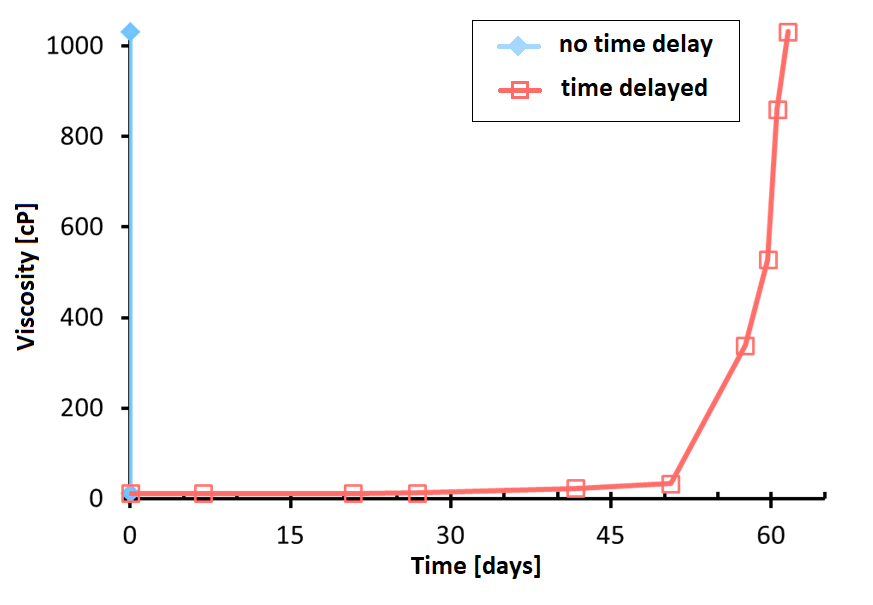
\includegraphics[width=.75\textwidth]{fig/jennTai.png}
    \caption{System with delayed gelation based on Texas A\&M technology \citep{Cordova2008}}
    \label{cht:jennTai}
\end{figure}
    
Samples of different basic systems were prepared for measurement of viscosity development with time. This included systems with only \ce{Cr^3+}-ions as cross-linker, systems based on the original Texas A\&M recipe \citep{Cordova2008} and systems with active FN. Polymers of different molecular weight were used.
    
\subsection{Transport Properties of Nanoparticles and Polymers in Porous Media}
\citet{Lotsch1985} described the phenomena governing the transport of water additives in porous media, namely retention, adsorption and inaccessible pore volume (IPV). Based on this, several core flooding experiments were designed and conducted where deactivated FN particles and polymer were injected both separately and in mixtures into two sets of sandstones, namely Berea and Bentheimer \citep{Najafiazar2016}. The results indicate that polymer adsorption, polymer retention and IPV were generally reduced by the presence of nanoparticles. Adsorption, total retention and IPV were significantly higher in Berea compared to Bentheimer, for both polymer and nanoparticles. Adsorbed or otherwise retained polymer during injection was not released during following water floods, while the retained nanoparticles were partly released during subsequent water floods. Nanoparticles had negligible effect on rock permeability, while polymer significantly reduced rock permeability.

\subsection{Numerical Model}
A numerical model in was developed and tested with results from the core flooding experiments with deactivated FN particles and polymer. Simulations were also run using a synthetic data set where polymer viscosity depends on polymer concentration and the concentration and age of the injected nanoparticles (the time passed since injection).

% %%%%%%%%%%%%%%%%%%%%%
% EXPERIMENTAL
\section{Experimental}
\subsection{PEC Nanogel Formation}
\textbf{Gels with \ce{Cr^{3+}} as crosslinker.}
Three different polymers (all HPAM) were used in the experiments as summarized in Table \ref{tab:crGels}, where the product names, the producers and the approximate molecular weights are given. The concentrations used are also given. The polymers were always dissolved in synthetic sea water, SSW (cf. Table \ref{tab:sswComp}). The exact molecular weight of Flopaam 5115 VHM is not known but assumed to be in the order of 12 - 15 MDa.

\begin{table} 
\centering
\caption{Basic rock parameters and additives used in the experiments.}
\label{tab:crGels} % table 5.1
\begin{tabular}{c c c c } 
\toprule
\textbf{Name} & \textbf{Producer} & \textbf{MW} & \textbf{Concentration} \\ 
&& [MDa] & [wt\%]   \\
\midrule 
Alcoflood 254 S     & BASF    & 0.5 & 0.5, 1.0 and 2.0\\
Alcomer 24 UK       & BASF    & 6 & 0.25, 0.5, 1.0 and 2.0  \\ 
Flopaam 5115 VHM    & SNF Floerger    & 12 - 15 & 0.5, 1.0 and 2.0  \\ 
\bottomrule
\end{tabular}
\end{table}

\begin{table} 
\centering
\caption{Composition of synthetic seawater (SSW)}
\label{tab:sswComp} 
\begin{tabular}{r c } 
\toprule
\textbf{Salt} & \textbf{Concentration} \\
& [g/l]\\
\midrule 
\ce{NaCl}       & 23.612\\
\ce{CaCl2.2H2O} & 1.911 \\ 
\ce{MgCl2.2H2O} & 9.149 \\ 
\ce{KCl}        & 0.746 \\
\ce{Na2SO4}     & 3.407 \\ 
\bottomrule
\end{tabular}
\end{table}

\textbf{Polyelectrolyte complexes according to the Texas A\&M recipe \citep{Johnson2010}.}
A few tests were conducted with PEC systems made after the recipe by Johnson et el \citep{Johnson2010}, in order to reproduce similar results. In this recipe which has three constituents, in addition to the polymer and cross binder \ce{Cr^3+} the main constituents are dextran sulphate (DS) \index{dextran sulfate} and polyethyleneimine (PEI)\index{polyethyleneimine}.
% The structure of the two polyelectrolytes are shown in Figure \ref{fig:pei}.
Each molecule consists of n repeated units, but n is different for the two components. 1 wt.\% of both components in pure water were prepared for making PEC solutions by adding 15.39 g of DS solution to 34.28 g of PEI solution under vigorous stirring. The DS solution was added quickly as a ``shot" by use of a syringe.

% \begin{figure}[h]
%     \centering
%     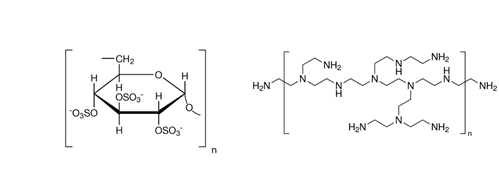
\includegraphics[width=\textwidth]{fig/pei.png}
%     \caption{Structures of dextran sulphate (DS) (left) and polyethyleneimine (PEI) (right).}
%     \label{fig:pei}
% \end{figure}    

 
After approximately one minute of stirring, 1.13 g of a 10 wt.\% \ce{CrCl3.6H2O} was added. The final solution was made by first mixing 5.38 g of a 4 wt.\% Alcomer 24 UK solution (in SSW\index{synthetic sea water}) with 25.35 g of SSW. Next, this polymer solution was mixed with 12.32 g of the PEC solution. The concentration of polymer and \ce{Cr^{3+}} in the final solution were 0.499 wt.\% and 129 ppm, respectively. The samples were aged at 50~\celsius. The sample series was named Series 10. The viscosity of the samples in each series was measured against increasing aging times. 

Two more series of polymer/PEC solutions were made using 0.498 wt.\% and 0.490 wt.\% of Alcomer 24 UK (Series 35) and Flopaam 5115 VHM (Series 36), respectively. The composition of the PEC was as described above. The concentrations of \ce{Cr^{3+}} in the two solutions were 119 ppm and 115 ppm. The solutions were aged at 80~\celsius. Yet another two systems were made in an equivalent manner using Alcomer 24 UK, but with reduced concentrations of \ce{Cr^{3+}} (60 ppm in Series 42 and 41 ppm in Series 47).

\textbf{Polyelectrolyte complexes based on amine POSS.}
In PECs based on amine POSS (Polyhedral Oligomeric Silsesquioxane) the polycation PEI was replaced by the nanoparticle which also contains amine groups. As suggested by researchers at Texas A\&M the DS was replaced by the polyanion polyvinyl sulfonate (PVS). As a result, the number of main constituents of PEC drops to two. Series 17 through 20 were made using this method (Table \ref{tab:polyPecComp}). The structure of PVS is also shown in Figure \ref{fig:pvs}.

\begin{figure}[h]
    \centering
    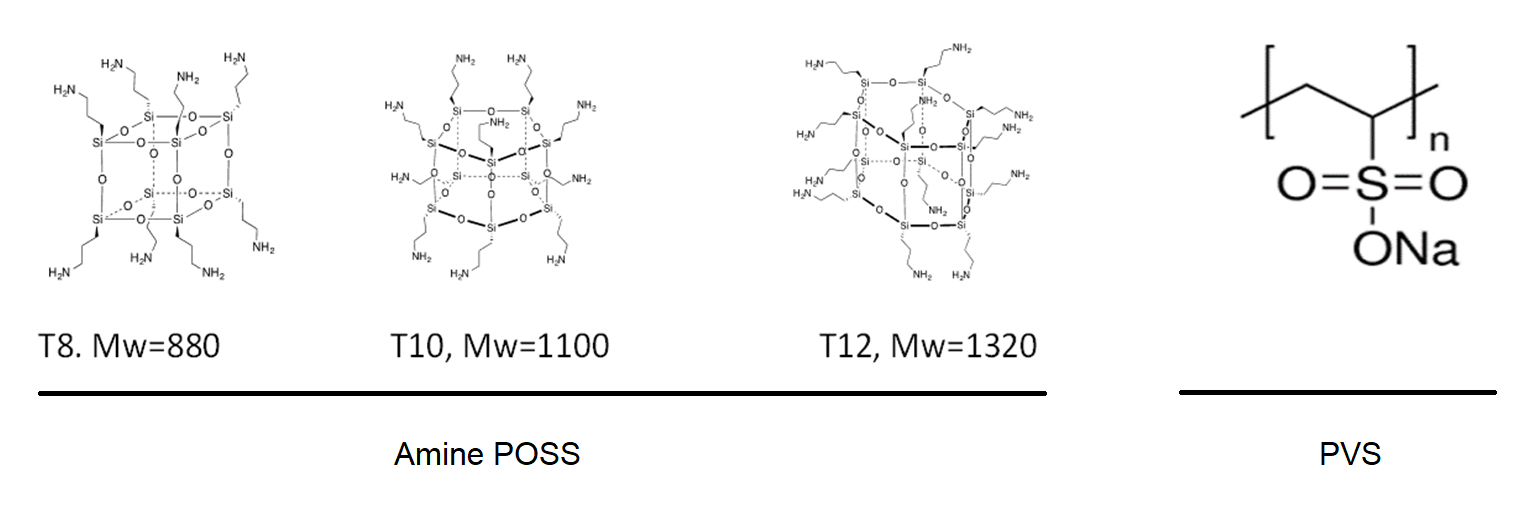
\includegraphics[width=\textwidth]{fig/pvs.png}
    \caption{Structures of amine POSS (left) and PVS (right).}
    \label{fig:pvs}
\end{figure}

The cores of the amine POSS are silicon oxide. The structure of the cores varies with the configurations shown in the figure, giving different molecular weights of the POSS particles. The amide POSS particles used in the samples were labelled FN 161128 and was 64.63 \% active matter in solvent.

Alcomer 24 UK was used as polymer. The composition of the samples are summarized in Table \ref{tab:polyPecComp}. The solvent for the solutions was SSW.

\begin{table} 

\centering
\caption{Composition of polymer/PEC sample series, concentraitons in weight \%}
\label{tab:polyPecComp}
\begin{tabular}{c c c c c c } 
\toprule
\textbf{Sample} & \textbf{$C_{Polymer}$} & \textbf{$C_{FN}$} & \textbf{$C_{PVS}$} & \textbf{$C_{pol}/C_{FN}$} & \textbf{$C_{FN}/C_{PVS}$} \\ 
&[wt\%]& [wt\%] & [wt\%] && \\
\midrule 
Series 17   & 1.002   & 0.380 & 0.053 & 2.64 & 7.16\\
Series 18   & 1.004   & 0.381 & 0.136 & 2.64 & 2.80\\ 
Series 19   & 0.931   & 0.382 & 0.273 & 2.64 & 1.29\\ 
Series 20   & 1.000   & 0.436 & - & 2.30     & - \\
\bottomrule
\end{tabular}
\end{table}

\textbf{Gels based on lactamide POSS.}
The solutions used in the core flooding experiments were prepared by mixing 500 g of 2 wt.\% Alcoflood 24 UK with 17.35 g of the lactamide POSS FN-LA-65-170210-1. The nanoparticles were supplied as a 90.59 \% active solid.

During the core flooding experiments the nanoparticle/polymer solution was injected into the SSW saturated cores. The viscosity of the effluent was monitored. As soon as the effluent viscosity had stabilized, a series of samples were taken. After collection and argon-purging, the samples were aged at 80~\celsius. 


\subsection{Aging}
Each prepared system was distributed into six vials (a through f) that were sealed with rubber stoppers and crimp seals. Then the vials were placed on a KS 500 shaker (Janke \& Kunkel, IKA WERK) with 300 shakes/min. While being shaken, the vials were purged with argon for 60 minutes. Argon was delivered through a syringe needle penetrating the rubber gasket. It then exited the vial through another needle.

After the purging, samples were placed in an oven and were heated to 50~\celsius~(the first 16 series) and later at 80~\celsius. The ``a" sample from each series was not heated, and its viscosity was measured a short time after preparation. Samples ``b" through ``f" were kept in the oven, each for an exponentially increased aging time. 

\subsection{Viscosity measurement}
The viscosities of samples were measured using an Anton Paar MCR 302 rheometer under ambient conditions. After a sample was taken out of the oven, it was quickly transferred to the rheometer station, after which its viscosity was measured using a plate and cone geometry.

The measurement procedure using the rheometer is as follows. First, a sample of suitable size was put on the plate. After that, the cone was lowered down onto the sample, until the sample spread into a thin film which completely filled the space between the cone and the plate. The measurement was then started according a preset schedule for shear rates. 

After initiating measurements, the instrument imposed a torque on the plate by rotating the cone at an initial slow speed, which was necessary to apply the first shear rate. The rotation lasted for the measurement time which was set to 2 seconds. After the measurement time had elapsed, the torque was increased to reach the next shear rate. From the resulting torques and shear rates a relationship between viscosity and shear rate (shear curve) was then calculated by the software.

\subsection{Effect of in-situ gelling on water flow}
Effect of in situ gel formation on water flow was studied. The gel system used in the experiments was the system developed at SINTEF DMN. The chosen system was considered the most promising with regard to delayed gelation and formation of strong gels.  The composition of the injected fluid is given in Table \ref{tab:injComp}. 
\begin{table} 
\centering
\caption{Composition of injected fluid}
\label{tab:injComp}
\begin{tabular}{c c c l } 
\toprule
\textbf{Constituent} & \textbf{Type} & \textbf{Mass} & \textbf{Comment}\\ 
&& [g] & \\
\midrule 
Polymer & Alcoflood 254S & 10.00 & MW $\thicksim$0.5 MDa, from BASF\\
Nanoparticles & FN-LA-65-170210 & 17.33 & 90.59 \% active matter \\ 
SSW & see Table \ref{tab:sswComp} & 490.0 &  \\ 
\bottomrule
\end{tabular}
\end{table}

The nanoparticles were added to the polymer solution and stirred overnight with a magnetic stirring bar. The solution was then filtered through 8\micro m membrane filters using less than 2 bar overpressure. The loss of solids during filtration (measured for one solution) was 0.74 \% of active matter in the solution. This was obtained by weighing of the filters before and after (dried filters) filtration. The filters clogged during filtration and five filters were used during the filtration.

The experiments were carried out in the setup shown in Figure \ref{fig:experimentalSetup} but the various detecting systems except for the viscometer were bypassed. The experiments were done using 20 cm long Bentheimer sandstone cores at 80~\celsius~ and 4 - 5 bar back pressure.

\begin{figure}[]
        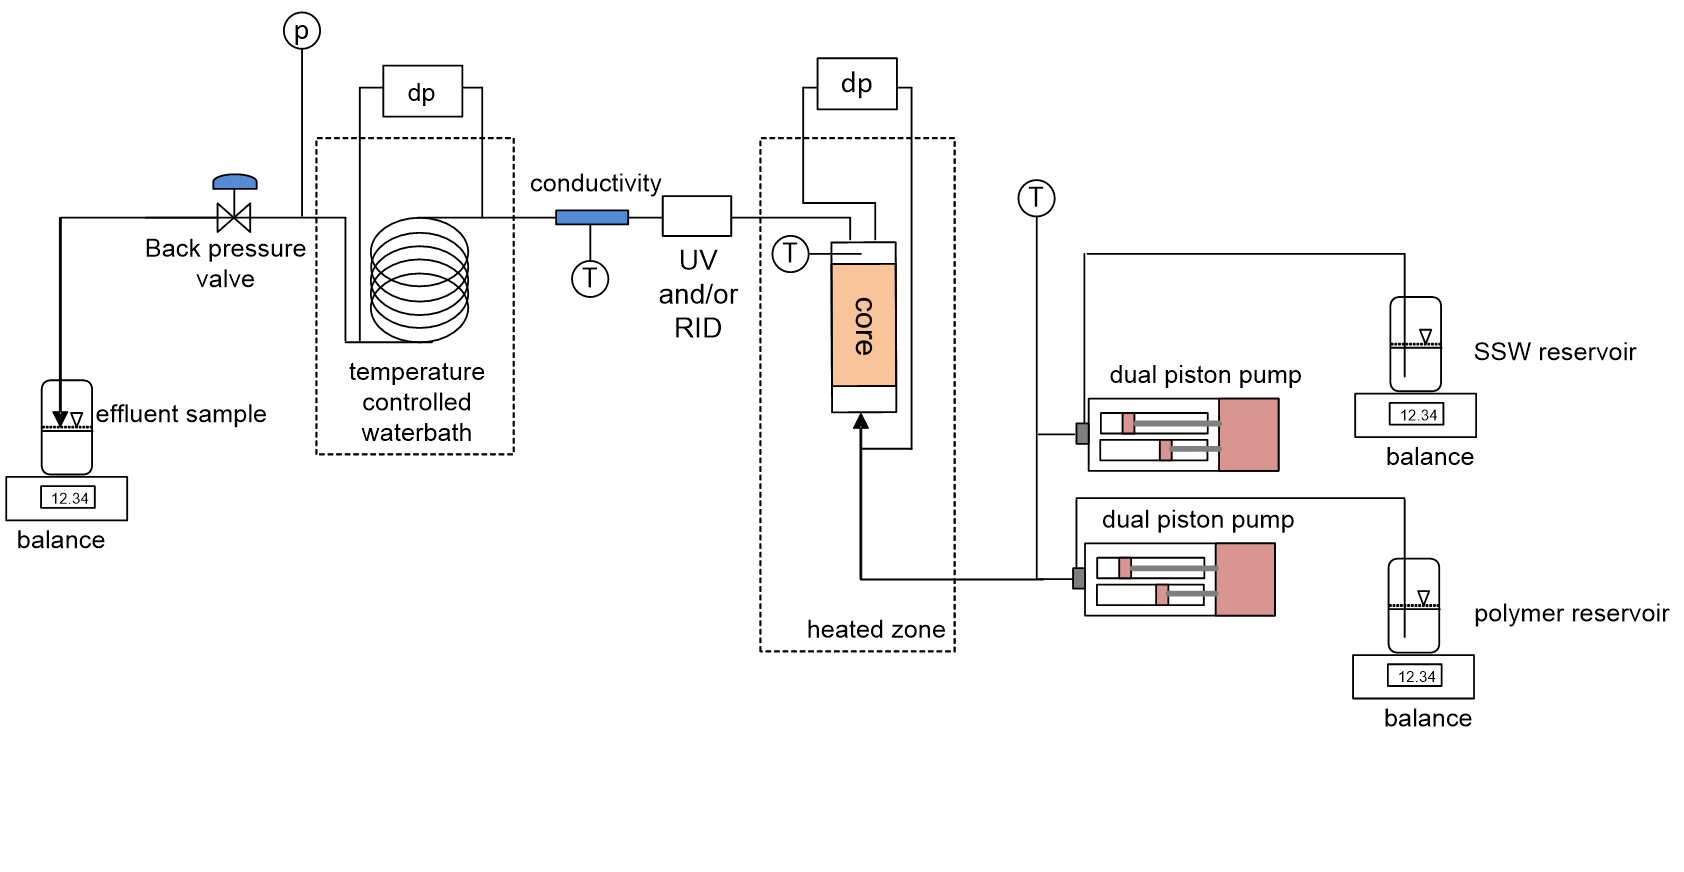
\includegraphics[width=\textwidth]{fig/experimentalSetup.png}
        \caption{Schematic of the setup of the core flooding experiments.}
        \label{fig:experimentalSetup}
\end{figure}

The Bentheimer cores were initially characterized by measurement of porosity and permeability. Pore size distribution was not measured for the present cores. However, from previous measurements with Bentheimer sandstones with the same porosities, a pore size distribution curve was determined based on mercury intrusion measurements. The curve was symmetrical around 33 \micro m with a peak of 0.43 ml/g differential intrusion, and only 11 \% of the pore throats were less than 10 \micro m.

% \begin{figure}
%     \centering
%     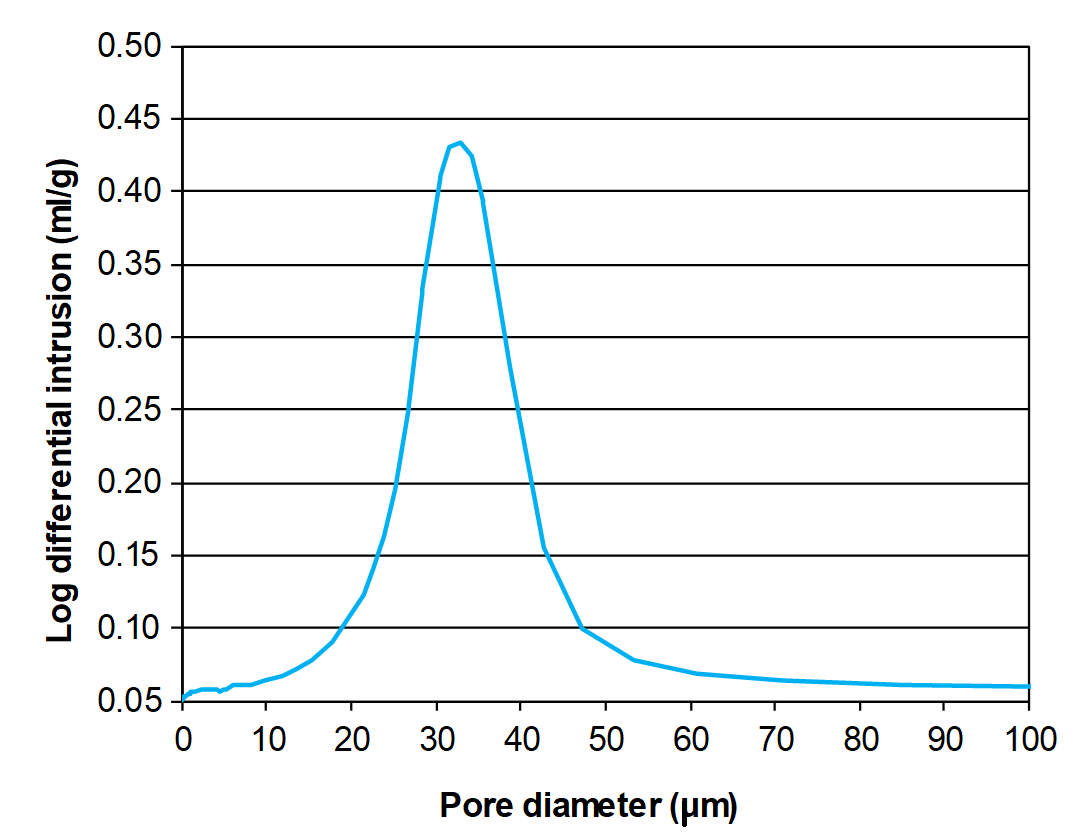
\includegraphics[width=.7\textwidth]{fig/poreSizeDist.png}
%     \caption{Pore size distribution for Bentheimer sandstone}
%     \label{cht:poreSizeDist}
% \end{figure}

The first three experiments were conducted with increasing aging times for the chemical system in the core. For each experiment, the pore volume and absolute permeability was first measured. Then, the chemical system was injected, followed by aging. After aging, SSW was injected at 30 ml/hr, and the experiments ended with a permeability measurement. During injection of the chemical system, samples of the produced fluid were taken early after breakthrough of the chemicals and at the end of the injection. The SSW injected prior to the polymer/nanoparticle solution was purged with argon and vacuum treated to remove oxygen from the solutions.

As differential pressures across the core increased significantly during injection of the identical nanoparticle/polymer solutions 2 more experiments were conducted. Experiment 4 was an injectivity test, pre-treating the injected solution by filtering it through a Berea sandstone. A last experiment was carried out by aging the solution with a more comprehensive pre-treatment, where:
\begin{itemize}
    \item the pH of the solution was adjusted to lower pH,
    \item the solution was filtered through filters with smaller pore size.
\end{itemize}

\section{Numerical Simulation}
\subsection{The Model}
A spatially 1-dimensional model with rate-controlled injection was developed. Thus, the model is most appropriate for simulation of core flooding experiments with specified injection rates. At present, the given version of the model does not contain capillary forces nor gravity. However, the formulation of transport properties can be generalized to more spatial dimensions, to include capillary forces and gravity, and to include the possibility of pressure-controlled boundary conditions. 

The model also contains other features (in addition to age tracking of nanoparticles) such as adsorption and possible desorption of nanoparticles and polymers, inaccessible pore space for nanoparticles and polymers, shear thinning, and absolute permeability reduction as a function of adsorbed polymer concentration. 

The water viscosity at a given location and time is a function of polymer concentration, nanoparticle concentration, the local age profile of the nanoparticles, as well as the rate. With no nanoparticles present, the formulation of the water viscosity as a function of polymer concentration corresponds to the fully mixed Todd-Longstaff formulation. When gelling is possible (i.e. when sufficiently aged nanoparticles and polymers are present), the water viscosity is interpolated between its value corresponding to no gelling and its maximal possible value (maximal gelling).  For generality, several of the input parameters defining water viscosity in the developed code are table based, allowing for flexibility in the definition of rheological properties of the water.

The numerical formulation of the presented model is standard upstream implicit Euler for the transport of water, oil, polymers, and nanoparticles, while the recalculation of the nanoparticle age distributions is done after the implicit transport equations have converged. This recalculation applies a relatively novel method \citep{Flatten2008} by treating the upstream terms explicit and the downstream terms implicit. This approach givens stability and limited dispersion. 

Since the model is spatially 1-dimensional, the Jacobian matrix in the Newton iteration has a block structure enabling a non-iterative robust and effective linear solver. Indeed, numerical simulations demonstrate robust stability due to the implicit formulation for fluid transport, and the simulator is numerically effective allowing for short timesteps in order to limit numerical dispersion inherent in the implicit formulation.

% \section{Transport of polymer and nanoparticles through porous media}
% \subsection{Experimental setup}
% A schematic of the experimental setup is shown in Figure \ref{fig:experimentalSetup}. To the right of the setup there were reservoirs containing either SSW, nanoparticle solution, polymer solution or mixtures of the latter two. The solutions were then pumped by a dual piston Pharmacia P-500 pump, and injected into the bottom of the vertical oriented core. The core itself was wrapped in nickel foil and inserted into a Viton rubber sleeve, around which a net overburden pressure of 50 bar was exerted. This ensured that no side flow occurred around the core and the metal foil prevented the sleeve pressure gas to diffuse through rubber sleeve.

% \begin{figure}[hp]
%     \adjustbox{minipage=\textheight,angle=90}{
%         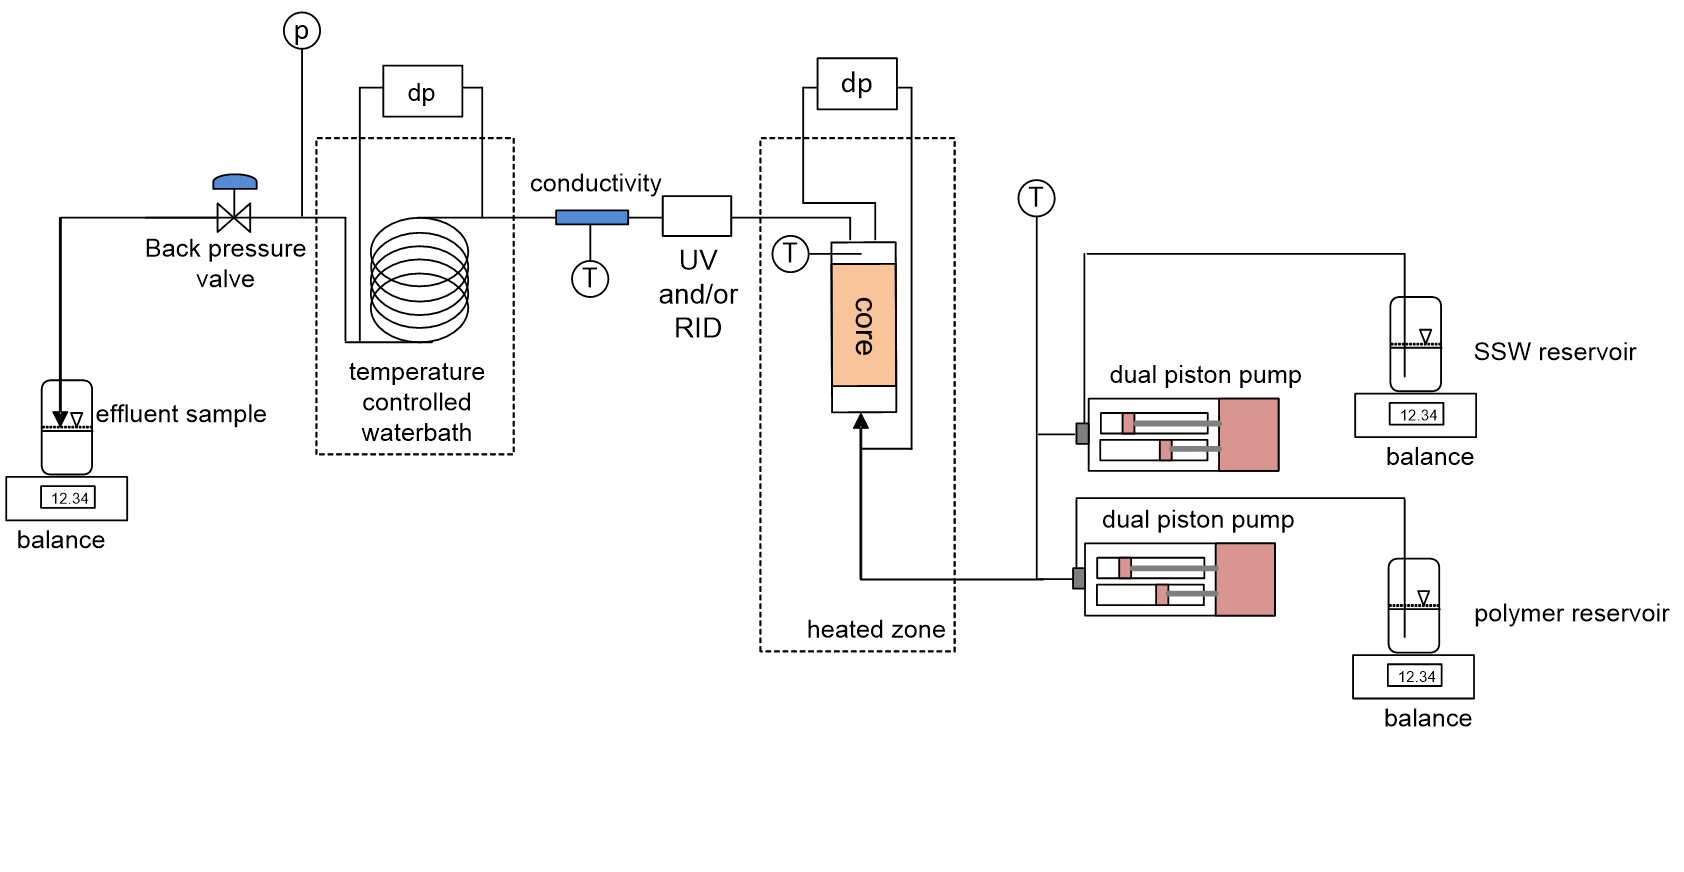
\includegraphics[width=\textwidth]{fig/experimentalSetup.png}
%         \caption{Schematic of the setup of the core flooding experiments.}
%         \label{fig:experimentalSetup}
%     }
% \end{figure}

% Several online measurement systems were placed downstream of the core. Conductivity of the effluent was measured by a Radiometer CDM 83 Conductivity Meter, determining the resistance of the fluid between two small rodded platinum electrodes integrated in a flow channel in a small housing made of polyoxymethylene. Since conductivity is substantially affected by temperature, these readings were temperature corrected. Viscosity of the effluent was measured by a spiral viscometer of 1/16" outer diameter. In order to avoid temperature effects, the viscometer was submerged in a water bath with a constant temperature. A refractive index detector (Shodex RI SE-51) and UV detector (KNAUER Azura MWD 2.1L) were employed interchangeably, in order to determine nanoparticle concentration. Several pressure transducers were implemented along the system. A back pressure of 3 – 6 bar was applied. To the left side of the experimental setup, the effluents were collected and weighed. The core temperature was at ambient for the experiments described in this section.

% \subsection{Core flooding experiments with polymer and/or inactive FN particles}

% First, a new core of diameter 3.8 cm and length 20 cm, was mounted in the core holder. After leakage testing of the system, the core was flooded with isopropanol until full saturation. Next several PVs of synthetic seawater (SSW) were flooded through the core in order to displace the isopropanol and ensure stable flow conditions. After that, porosity and permeability measurements were conducted. Porosity was measured by NaNO3 flooding of the SSW saturated core. The concentration of \ce{Cl-} in the collected fluid was determined by potentiometric titration. The pore volume (PV) was calculated from the total amount of chloride, adequately corrected for dead volumes.

% Each experiment started with injection of a slug with only nanoparticles, only polymer or a mixture of nanoparticles and polymer (Stage 1). After some time, the measurements stabilised. In Stage 2, the injected fluid was switched to pure brine (with lower salt concentration in the experiments only involving polymer) and the injection continued until the measurements became stable. In Stage 3, a second slug with additives was injected, followed by a second slug with only brine (Stage 4). In other words, stages 3 and 4 were a repetition of stages 1 and 2. All stages ran until measurements became steady state. The experiment ended with a final water permeability measurement. During the experiment, process parameters and detector/sensor readings were continuously logged.

% Quantification of produced polymer and nanoparticles was carried out using the viscosity measurements and/or measured changes in refractive index and UV absorption. Figure \ref{cht:uv} shows calibration models for UV absorption and pressure drop in the viscometer tube. As seen in the figure, the pressure drop over viscometer tube is practically only affected by polymer concentration, giving a second order model in polymer concentration. Viscosity measurements alone were therefore used to find the concentration of produced polymer. On the other hand, UV absorption data resulted in a model with first and second order terms with respect to both nanoparticles and polymer, as well as a cross term (i.e., the product of concentrations). Similar responses were also found for changes in refractive index. UV absorption measurements and changes in refractive index were used to generate nanoparticle responses. For the experiments that involved nanoparticles, the conductivity responses were determined in separate runs from the main core floods. This was because changes in salt concentration affected both UV absorption at low wavelengths and especially the refractive index of the fluid. The conductivity responses were measured with the same injection rates with slugs of SSW and 80\% SSW into the cores.

% \begin{figure}[h]
%     \centering
%     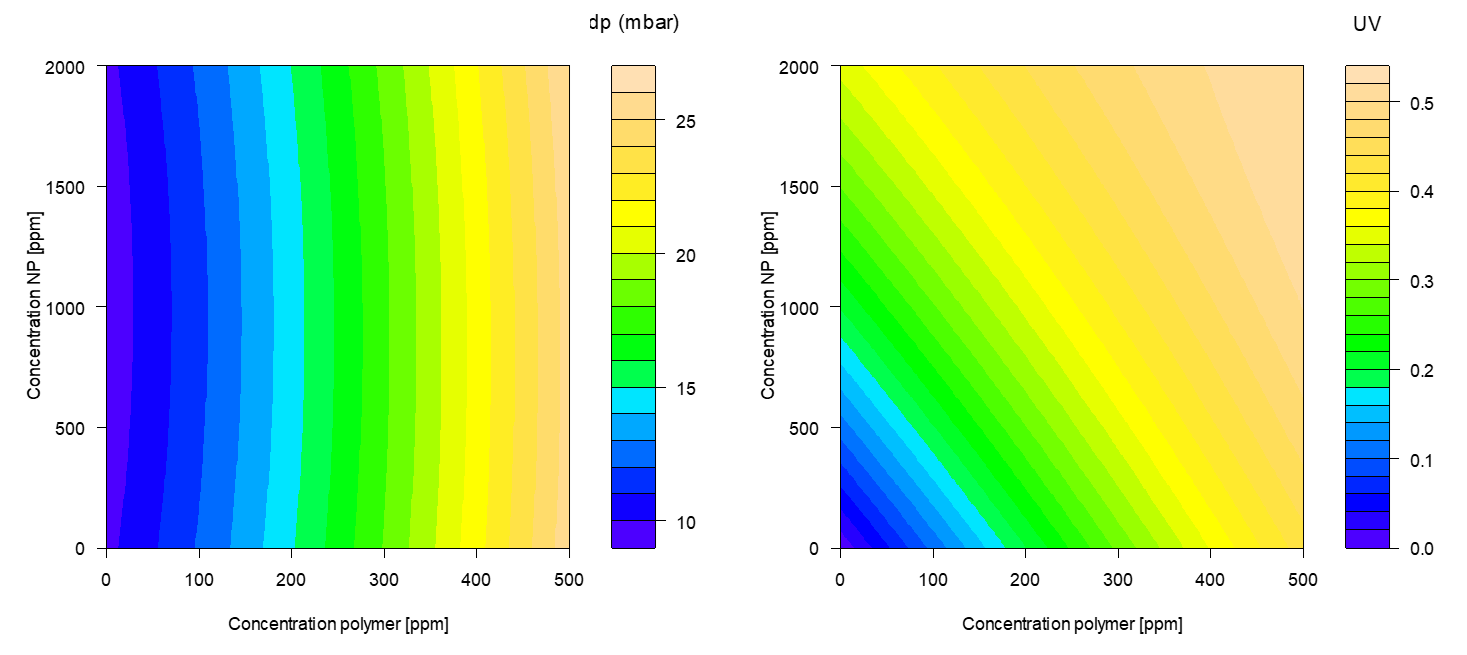
\includegraphics[width=\textwidth]{fig/uvDetector.png}
%     \caption{Calibration models for pressure drop in viscometer (left) and UV absorption in UV detector (right). Polymer concentration varies along the horizontal axis and nanoparticle concentration varies along the vertical axis.}
%     \label{cht:uv}
% \end{figure}

% Online measurements of polymer and nanoparticles using UV and refractive index measurements proved to be difficult. The reason for this is not revealed, but staining of the flow cells in the instruments is believed to be the most likely cause of these problems that also affected the accuracy in the results.

% Nanoparticle and polymer solutions were prepared with synthetic SSW as solvent. Table \ref{tab:rockParams} summarizes the six different additive combinations used. Some of the experiments were repeated. Table \ref{tab:sswComp} shows the recipe for SSW used. In order to make a nanoparticle solution, Funzio-nano particles (FN-PEGMEA-100-141128) produced at SINTEF Materials and Chemistry were dissolved in SSW using a magnetic stirrer and then exposed to ultra-sonic bath a better dissolution. Finally, the solution was filtered through a 0.45 µm membrane filter. No significant increase in mass of the filters were detected. Partially hydrolyzed polyacrylamide (HPAM, FP 5115 VHM from SNF Floerger) was employed as the polymer. The molecular weight of the polymer is not exactly known but assumed in the order of 12 - 15 MDa. HPAM powder was dissolved in SSW with a propeller at 500 rpm followed by magnetic stirring. The polymer solutions, either at working concentrations or more concentrated solutions, were filtered through 5 cm long 500 mD Berea cores at rates up to 16 ml/min, but avoiding differential pressures over 20 bar. Two types of sandstone were used; Berea and Bentheimer. Basic core parameters are given in Table \ref{tab:rockParams}.

% \begin{table} 
% \small
% \centering
% \caption{Basic rock parameters and additives used in the experiments.}
% \label{tab:rockParams}
% \begin{tabular}{c c c c l } 
% \toprule
% \textbf{Exp. no.} & \textbf{Rock} & \textbf{Permeability} & \textbf{Porosity} & \textbf{Additive} \\ 
% && [Darcy] & [\%] & \\
% \midrule 
% 1   & Bentheimer    & 2.74 & 23.1 & Nanoparticles\\
% 2   & Bentheimer    & 2.81 & 23.1 & Polymer \\ 
% 3   & Bentheimer    & 2.84 & 23.5 & Nanoparticles \& Polymer \\ 
% 4   & Berea      & 0.365 & 19.7 & NanoParticles\\
% 5   & Berea      & 0.288 & 18.6 & Polymer \\ 
% 5   & Berea      & 0.359 & 19.7 & Nanoparticles \& Polymer \\ 
% \bottomrule
% \end{tabular}
% \end{table}


% % % %%%%%%%%%%%%%%%%%%%%%
% % % RESULTS
\section{Results and Discussion}
\subsection{Laboratory Experiments}
\textbf{Gel Formation Experiments.} Table \ref{tab:crGelsAt} shows the lowest concentration for gel formation with the different polymers used in the experiments with \ce{Cr^{3+}} as the crosslinker. As seen the table, gel was only formed with Alcoflood 254 S for the highest concentration tested, namely 2 wt.\%. However, it is possible that gels could have been formed at lower concentrations in the interval between 1 wt.\% and 2 wt.\%. Alcomer 24 UK formed gel at 0.5 wt.\% but not at 0.25 wt.\%. It is possible that the highest molecular weight polymer Flopaam 5115 VHM could have formed gels at concentrations lower than 0.5 wt.\%.

Samples prepared according to published Texas A\&M technology showed that it was possible to delay gelation for in the order of 20 days when the sample was aged at 50~\celsius. At 80~\celsius~ the gelation was much faster, comparable to systems cross-linked with only Cr3+.

% Figure \ref{cht:s10visc50} shows viscosity as function of time on logarithmic and linear scales. As shown in the figure, there were only minor increases in viscosity the first 7 days. After 23 days, the viscosity was increased significantly and it increased further when the last sample was measured after 37 days. Simple power functions were fitted to the experimental data. The plot on linear scale suggest that the largest effect of the cross binding occurred after approximately 20 days. 

% \begin{figure}
%     \centering
%     \makebox[\textwidth][c]{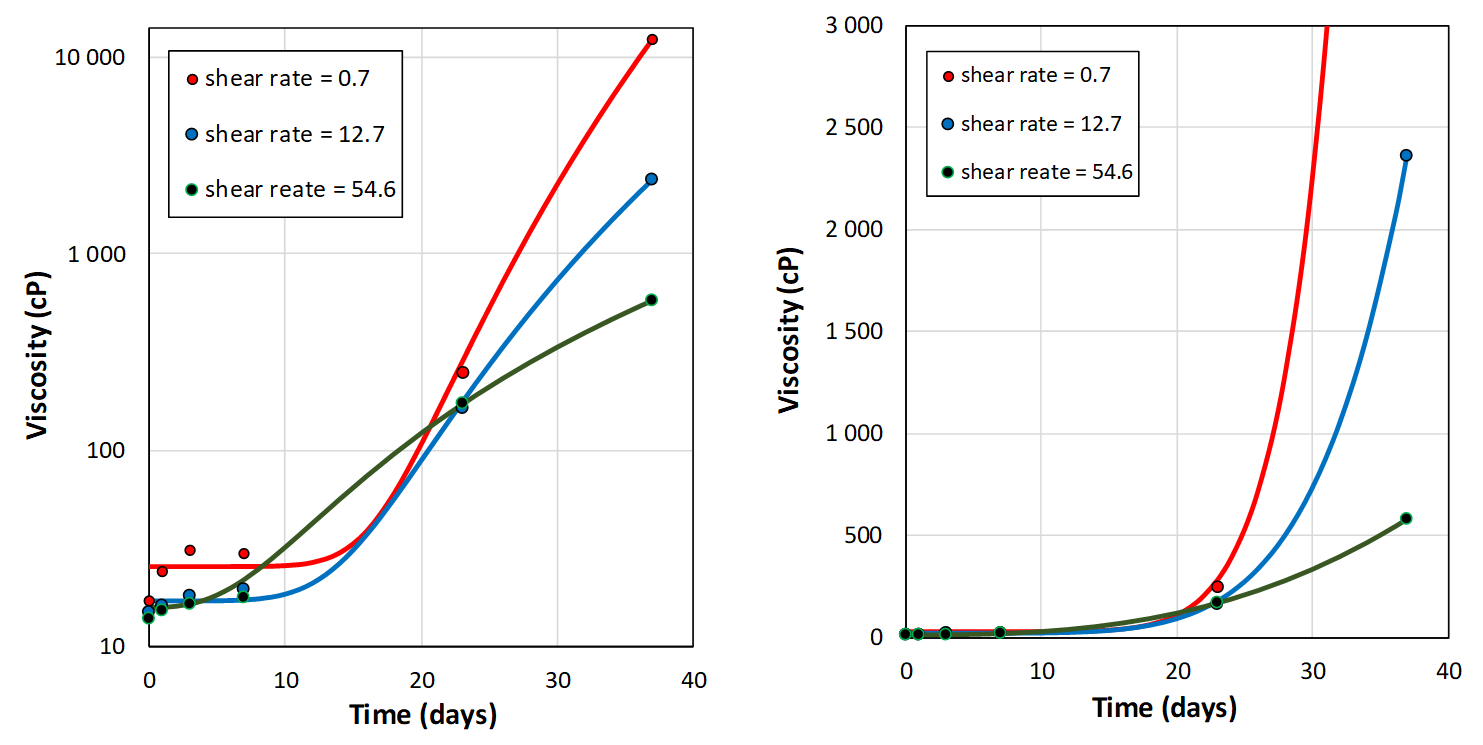
\includegraphics[width=\textwidth]{fig/s10visc50.png}}
%     \caption{Viscosity as function of aging time for Series 10 samples aged at 50~\celsius~ on logarithmic (left) and linear (right) scales}
%     \label{cht:s10visc50}
% \end{figure}

Figure \ref{cht:s23visc80} shows measured viscosities for the samples collected early and at the end of the injection during an experiment with gels based on lactamide. Except for the sample measured after 12 days at 0.7 s$^{-1}$, a clear trend is seen in the figure showing a slow increase in viscosity the first 25 days and then a faster increase thereon.

\begin{figure} 
    \centering
    \makebox[\textwidth][c]{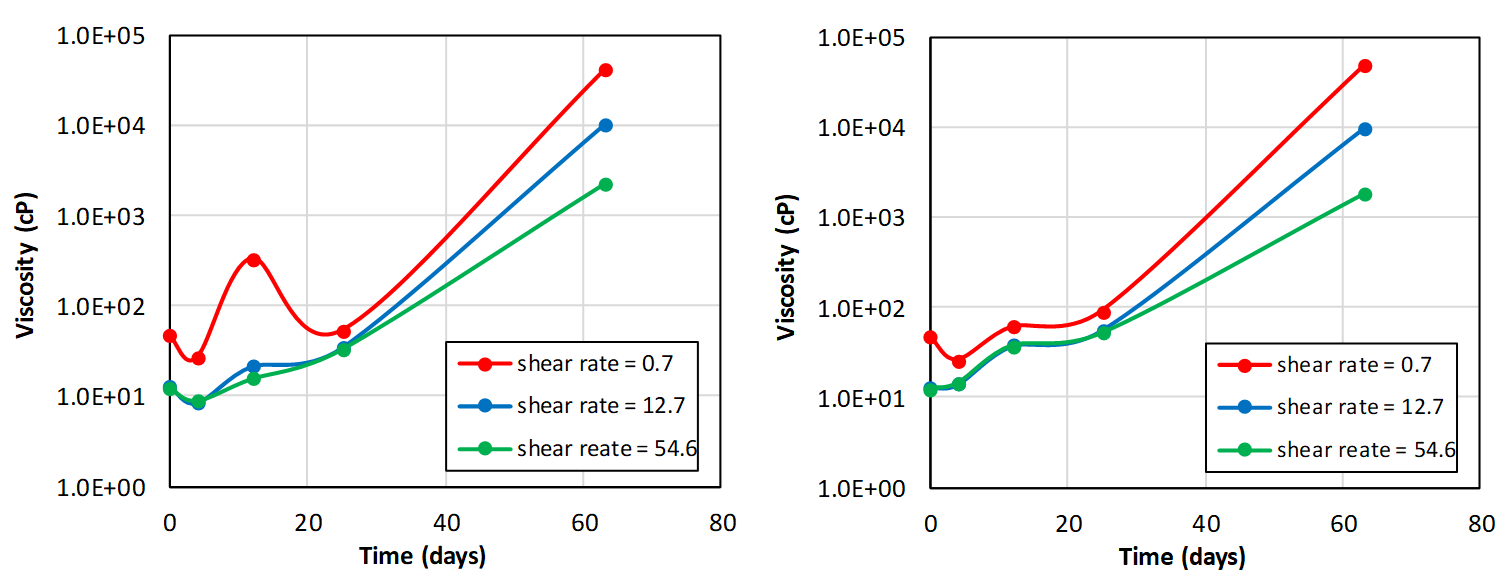
\includegraphics[width=\textwidth]{fig/s23visc80.png}}
    \caption{Aging of solutions in Series 23 collected during injection of nanoparticle/polymer solution in a core. Samples collected early (left) and collected at the end of the injection (right).}
    \label{cht:s23visc80}
\end{figure} 

Figure \ref{cht:s17visc80} illustrates the viscosity measurement results for gels based on PECs with amine POSS. The figure shows that on the first day of aging, the viscosities in all solutions increased to some degree. Then all three solutions with PEC (Series 17 through 19) exhibited an almost constant viscosity for 14 days. After 57 days, a significant increases in viscosity was seen for all the three solutions. After 14 days the samples in Series 17 through Series 19 were characterized as viscous fluids. The samples in Series 20 were prepared without PVS and thus without PEC. For this series, the solution was characterized as viscous fluid after 5 days and as week gel after 11 days. Comparison of the samples made with and without PEC shows that incorporation of the amine POSS in PEC reduced gel formation significantly. Surprisingly, no effect was observed by increasing the amount of PVS.

\begin{figure}
    \centering
    \makebox[\textwidth][c]{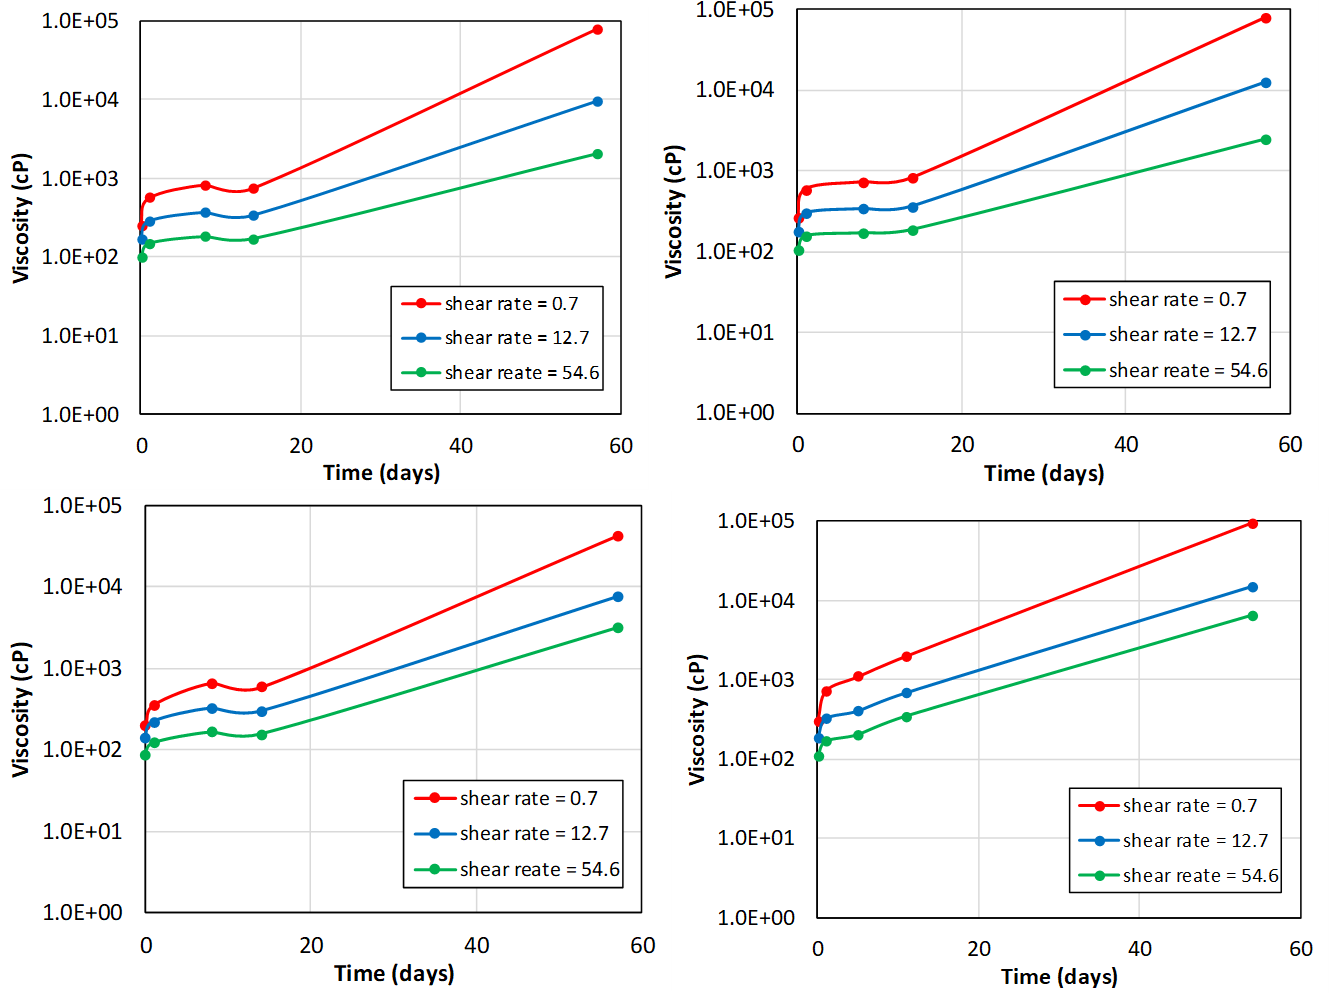
\includegraphics[width=\textwidth]{fig/s17visc80.png}}
    \caption{Polymer/PEC solutions aged at 80~\celsius. Upper left: Series 17 samples. Upper right: Series 18 samples. Lower left: Series 19 samples. Lower right: Series 20 samples.}
    \label{cht:s17visc80}
\end{figure}


In order to obtain data for testing of the simulator \--- developed for transport of nanoparticles and polymer, and with a functionality of time delayed gel formation \--- some gel formation experiments were conducted where the polymer concentration was varied from 0.25 wt.\% to 1 wt.\% and the concentration of \ce{Cr^{3+}} was varied from 22 ppm to 113 ppm. For this series of experiments, Alcomer 24 UK was used as polymer. For concentrations higher than 22 ppm, the polymer viscosity was apparently not dependent on the cross-binder concentration. The viscosities of the solutions were measured directly after preparation and after one day of aging. Figure \ref{cht:viscAlco} shows viscosity as function of shear rate for three polymer concentrations. 
\begin{figure}
    \centering
    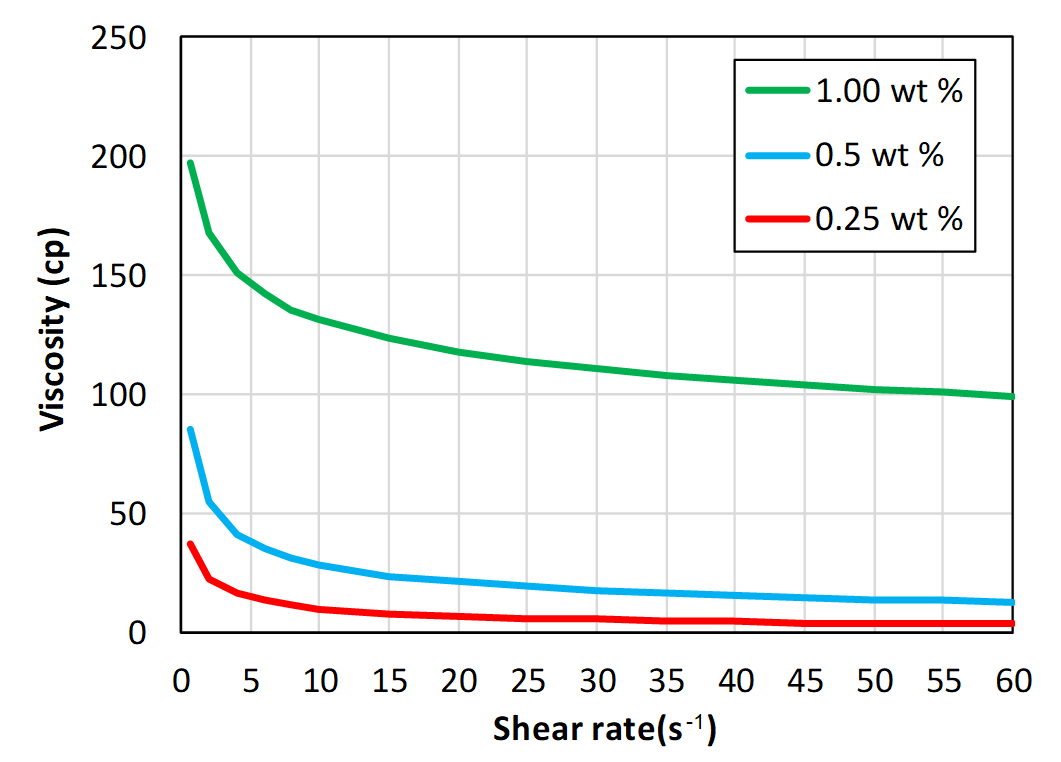
\includegraphics[width=.75\textwidth]{fig/viscAlcomer.png}
    \caption{Viscosity as function of shear rate and polymer concentration for Alcomer 24 UK}
    \label{cht:viscAlco}
\end{figure}

\begin{table}[h]
\small
\centering
\caption{Minimum concentration for gel formation for the different polymers with \ce{Cr^{3+}} as the crosslinker}
\label{tab:crGelsAt}
\begin{tabular}{c c c c >{\columncolor[gray]{0.8}}c } 
\toprule
\textbf{Name} & \textbf{Producer} & \textbf{MW} & \textbf{Concentration} & \textbf{Will gel at} \\ 
&& [MDa] & [wt\%] & [wt\%]  \\
\midrule 
Alcoflood 254 S     & BASF    & 0.5 & 0.5, 1.0 and 2.0 & 2\\
Alcomer 24 UK       & BASF    & 6 & 0.25, 0.5, 1.0 and 2.0 & $\geq 0.5$ \\ 
Flopaam 5115 VHM    & SNF Floerger    & 12+ & 0.5, 1.0 and 2.0 & $\geq 0.5$ \\ 
\bottomrule
\end{tabular}
\end{table}

Figure \ref{cht:viscPolcModel} shows an example of a reaction model designed based on viscosities measured at a shear rate of 12.7 s$^-1$ for the fresh made solutions and after one day of aging. The blue curve corresponds to the polymer which has not reacted, i.e. data taken from Figure \ref{cht:viscAlco}. It also corresponds to the viscosities for aging times less than 50 days with reference to Figure \ref{cht:jennTai} (although some viscosity increase was seen in this period). The red curve corresponds to maximum viscosities for the solutions, corresponding to the value after 60 days in Figure \ref{cht:jennTai} that is only valid for a single polymer concentration. The green curve is for aging time laying between no gelling and complete gelling. Again, with reference to Figure \ref{cht:jennTai} the green curve would be valid for an aging time of 55 days. In the reaction model, it is assumed that the viscosity increases linearly with time in the gelling period. Again, as mentioned above, the reaction model was solely made to have some reality based data to be used for testing of the simulator model. 

\begin{figure}
    \centering
    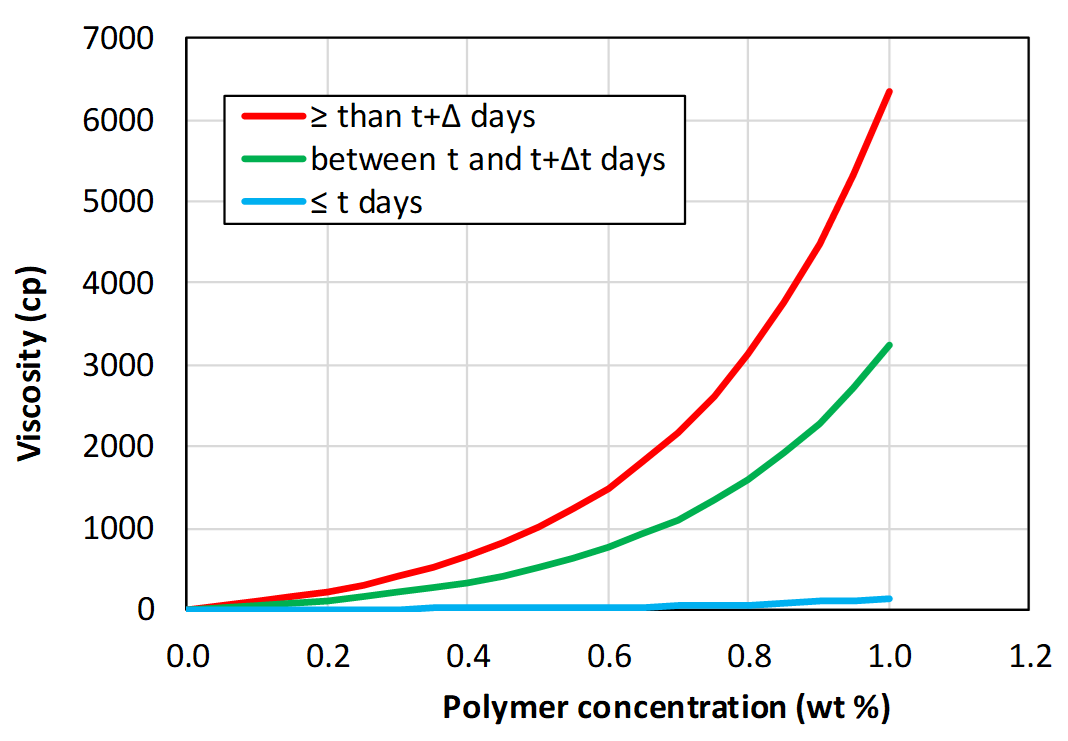
\includegraphics[width=.75\textwidth]{fig/viscPolcModel.png}
    \caption{Reaction model for Alcomer 24 UK}
    \label{cht:viscPolcModel}
\end{figure}

\textbf{In situ Gelling Experiments.}
Table \ref{tab:porPermAge} summarises the initial absolute permeabilities of the cores used in the experiments, the permeabilities measured after the SSW injections and the residual resistance factors, i.e. the ratio between the two permeabilities. The resistance factor determined after 7 days of aging was not much higher than the corresponding factor determined for polymer injection into Bentheimer sandstone. As shown in Table \ref{tab:porPermAge}, the residual resistance factors increased with longer aging times.
%TAB
\begin{table}
\small
\centering
\caption{Porosities, initial and final permeabilities and residual resistance factor for various aging times.}
\label{tab:porPermAge} % 5.12
\begin{tabular}{c l l l l l } 
\toprule
\textbf{Exp. no.} & \textbf{Porosity} & \textbf{Aging time} & \textbf{Abs. perm.} & \textbf{Residual perm.} & \textbf{RRF} \\ 
 & [fraction] & [days] & [mD] & [mD] & \\
\midrule 
1  & 0.221   &  7     & 2653     & 306      & 8.7    \\
2  & 0.221   & 23     & 2580     & 5.2      & 493      \\ 
3  & 0.221   & 66     & 2706     & 0.008    & 3230   \\ 
4  & NM* & Injectivity test & 2571    & -        & -      \\
5  & 0.224   & 53     & 2710     & 0.002        & 158000      \\
\bottomrule
* Not measured.
\end{tabular}
\end{table}

The injection phases for the nanoparticle/polymer solution are compared in Figure \ref{cht:gelexp_sum}. As seen the differential pressures across the viscometer tube were similar except for a slightly higher viscosity of the solution used in Experiment 5. In Experiment 3, parts of the bypass line was filled with the nanoparticle/polymer mixture, explaining the initial decline in the viscosity response. 

\begin{figure}[h!]
    \centering
    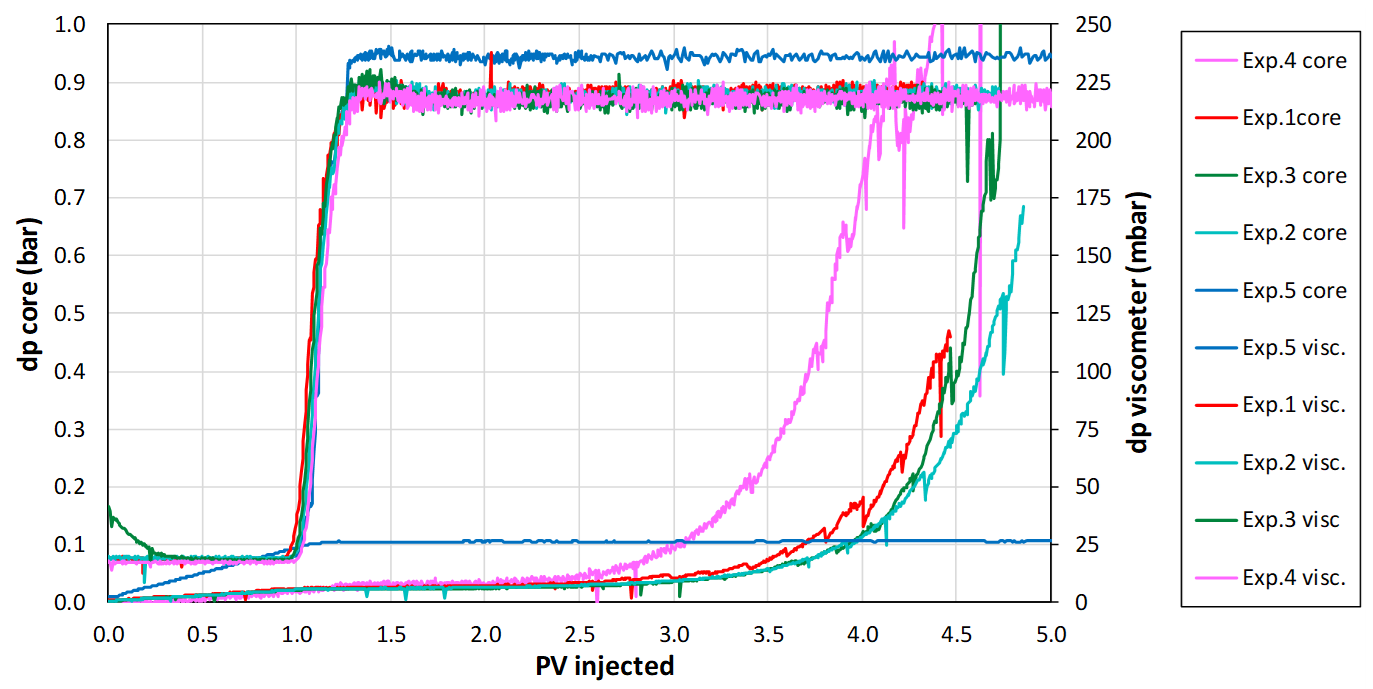
\includegraphics[width=\textwidth]{fig/gelexp_sum.png}
    \caption{Comparison of nanoparticle/polymer injection phases.}
    \label{cht:gelexp_sum} % 5.39
\end{figure}
 
The differential pressures over the core developed almost identical for the first 2.5 PVs injected. The rapid increase thereafter, developed in different, but quite similar manners. Pre-Filtering of the injected solution through a 500 mD core (Experiment 4) apparently gave a worse result compared to filtration through 8 \micro m membrane filters in Experiments 1 through 3.

If the presence of extended structures/particles in the solution was the cause of the injectivity problem, the use of finer filters could possibly alleviate the problem. In Experiment 5, the first half of the injected solution was filtered through 3 \micro m filters and the second half through 6 \micro m filters. Likely more important, the pH of the injected solution was reduced to 7.2 which resulted in a clear solution before filtering. 

As can be seen in Figure \ref{cht:gelexp_sum}, the differential pressure across the core did not increase after breakthrough of the nanoparticle/polymer solution in Experiment 5, and it remained stable until all available solution was injected (15.3 PV). The improved treatment thus alleviated the injectivity problem seen in the first four experiments.

The experiments with \textit{in situ} gelling has demonstrated that gel is formed in the porous medium. As expected the gel strength increases with increased gelling time. For gelling
times in the order of 2 months strong gels were formed. 

In Experiment 3, the gel almost blocked the core with a pressure gradient of 135 bar/m for almost 9 days at 80~\celsius. In Experiment 5, the gel blocked the core during the entire test period of 45 days using the same pressure gradient and temperature. At the end of Experiment 5 flow rate of SSW through the core was 0.23 ml/hr. 

It is evident that pH adjustment of the nanoparticle/polymer solution affected both the gelation rate and gel strength. The nanoparticle/polymer systems developed in the present project has proven the ability to delay gelation and form stable gels at harsh conditions. However, further work is needed in order to optimise the systems for use in practical applications. 

\subsection{Simulation of Laboratory Experiments}
Experiment 1 to 3 injects solutions of nanoparticles and polymer in SSW into a Bentheimer sandstone core with permeability around 2.8 Darcy and porosity around 23\% (see Table \ref{tab:crGels}).

Experiment 1, nanoparticle injection into Bentheimer sandstone, injects two slugs with 1000 ppm nanoparticle (NP) concentration dissolved in synthetic sea water (SSW) each followed by SSW without NP. Inaccessible pore volume (IPV) for nanoparticles is assumed to be zero and the measured retention (0.010 mg/g rock) are taken into the adsorption isotherm. It is assumed that desorption of nanoparticles occurs for SSW flooding based on negative IPV for the SSW flooding (see Table \ref{tab:ipvexp1}). Figure \ref{cht:simExpNP} shows comparison of nanoparticle response from the simulation and the experiment for injection of nanoparticles into Bentheimer sandstone.

\begin{table} % table 5.3
\small
\centering
\caption{Inaccessible pore volume (IPV) and retention of nanoparticles during Experiment 1.}
\label{tab:ipvexp1}
\begin{tabular}{c l l l l l } 
\toprule
\textbf{Quantity} & \textbf{Unit} & \textbf{Stage 1} & \textbf{Stage 2} & \textbf{Stage 3} & \textbf{Stage 4} \\ 
\midrule 
IPV         & [PV]          & -         & -0.03     & -         & -0.02     \\
Retention   & [mg]          & 4.3       & 2.5       & 5.8       & 4.7       \\ 
Retention   & [mg/g rock]   & 0.009     & 0.005     & 0.013     & 0.010     \\ 
Retention   & [mg/PV inj]   & 1.89      & -         & 0.96      & -         \\
Retention   & [\% of inj NP]& 3.6       & 2.0       & 1.8       & 1.5       \\ 
\bottomrule
\end{tabular}
\end{table}

\begin{figure}[h]
    \centering
    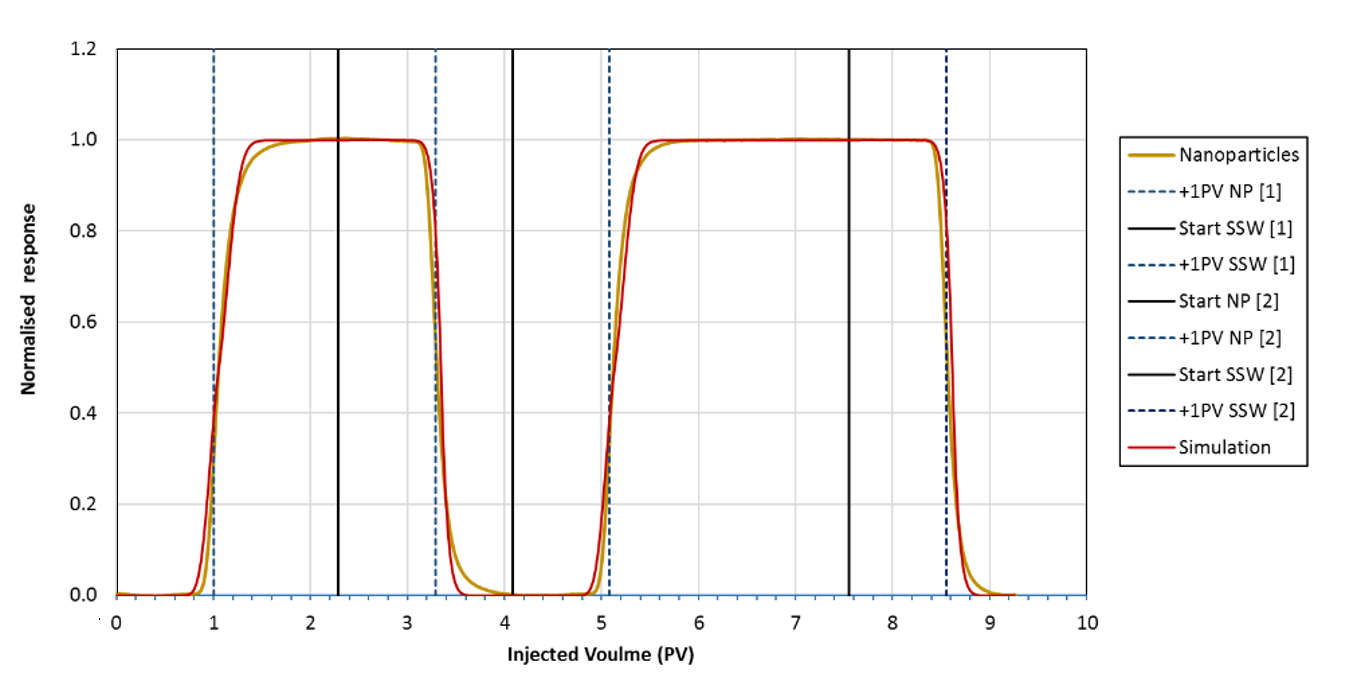
\includegraphics[width=\textwidth]{fig/simExpNP.png}
    \caption{Comparison of normalised nanoparticle concentration at the outlet of the core from experiment and from simulation of Experiment 1 (Bentheimer). The normalised nanoparticle response is plotted as function of injected PV.}
    \label{cht:simExpNP}
\end{figure}

Experiment 2, polymer injection into Bentheimer sandstone, injects two slugs of 1000 ppm polymer dissolved in SSW, each followed by SSW. For this case, an increase in viscosity as a function of polymer concentration and IPV for polymer is included in addition to adsorption of polymer on the rock surface. Adsorbed polymer also reduces absolute permeability in the rock. No desorption of polymer is assumed. Parameter input for the simulations are taken from Table \ref{tab:ipvexp2}, with IPV equal to 0.1 (average between 0.07 and 0.13) and adsorption coefficient at maximum polymer concentration equal to 0.02 mg/g rock (includes mechanical trapping). The reduction in absolute permeability for SSW with polymer is adjusted to match the differential pressure over the core. The viscosity of SSW as function of polymer concentration are taken from measurements giving a relative increase in viscosity by a factor of 4.31 at 1000 ppm polymer concentration. Figure \ref{cht:simExpNP2} shows comparison of normalised polymer response and differential pressure over the core/model from the simulation and experiment of polymer injection into Bentheimer sandstone.

\begin{table} 
\small
\centering
\caption{Inaccessible pore volume (IPV), adsorption and mechanical entrapment of polymer during Experiment 2.}
\label{tab:ipvexp2}
\begin{tabular}{c l l l l l } 
\toprule
\textbf{Quantity} & \textbf{Unit} & \textbf{Stage 1} & \textbf{Stage 2} & \textbf{Stage 3} & \textbf{Stage 4} \\ 
\midrule 
IPV                & [PV]           & -         & 0.07     & -         & -0.02     \\
Mech. entrapment   & [mg]          & 3.3       & 3.3       & 5.8       & 4.7       \\ 
Mech. entrapment   & [mg/g rock]   & 0.007     & 0.007     & 0.013     & 0.010     \\ 
Mech. entrapment   & [mg/PV inj]   & 0.74      & -         & 0.96      & -         \\
Mech. entrapment   & [\% of inj pol.]& 1.3       & 1.3       & 1.8       & 1.5       \\ 
Adsorption         & [mg]          & 4.8       &   \multicolumn{3}{c}{\multirow{2}{15em}{from difference in response curves of stages 1 and 3}}        \\
Adsorption         & [mg/g rock]   & 0.10      &  \multicolumn{3}{c}{}    \\ 
\bottomrule
\end{tabular}
\end{table}

\begin{figure}[h]
    \centering
    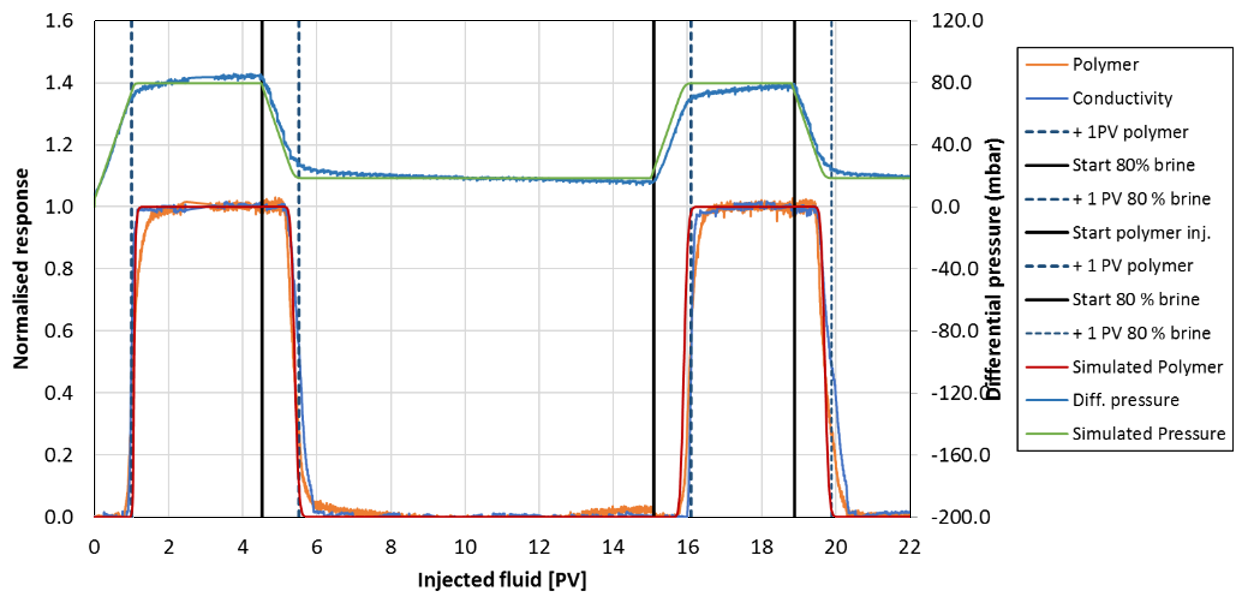
\includegraphics[width=\textwidth]{fig/simExpNP2.png}
    \caption{Comparison of normalised polymer concentration at the outlet of the core from experiment and from simulation of Experiment 2 (Bentheimer). Conductivity measurements from the experiment and differential pressure over the core is also plotted.}
    \label{cht:simExpNP2}
\end{figure}

Experiment 3 injects a solution with polymer and nanoparticles into Bentheimer sandstone. Two slugs with 2000 ppm nanoparticles and 500 ppm polymer were injected each followed by injection of SSW. Parameters for adsorption, IPV, permeability reduction and viscosity changes for nanoparticles and polymer are the same as for experiment 1 and 2, respectively. Figure \ref{cht:simExpNP3} shows simulation results compared to results from the experiment. Parameter input for the simulations are taken from Table \ref{tab:ipvexp3}.

\begin{table} 
\small
\centering
\caption{Inaccessible pore volume (IPV) and retention of nanoparticles during Experiment 3.}
\label{tab:ipvexp3}
\begin{tabular}{c l l l l l } 
\toprule
\textbf{Quantity} & \textbf{Unit} & \textbf{Stage 1} & \textbf{Stage 2} & \textbf{Stage 3} & \textbf{Stage 4} \\ 
\midrule 
IPV         & [PV]          & -         & -0.16     & -         & -0.08     \\
Retention   & [mg]          & 153       & 125       & 132       & 114       \\ 
Retention   & [mg/g rock]   & 0.35      & 0.28     & 0.30     & 0.26     \\ 
Retention   & [mg/PV inj]   & 0.47      & -         & 0.02      & -         \\
Retention   & [\% of inj NP]& 23        & 19       & 0.87       & 7.9       \\ 
\bottomrule
\end{tabular}
\end{table}

\begin{figure}[h]
    \centering
    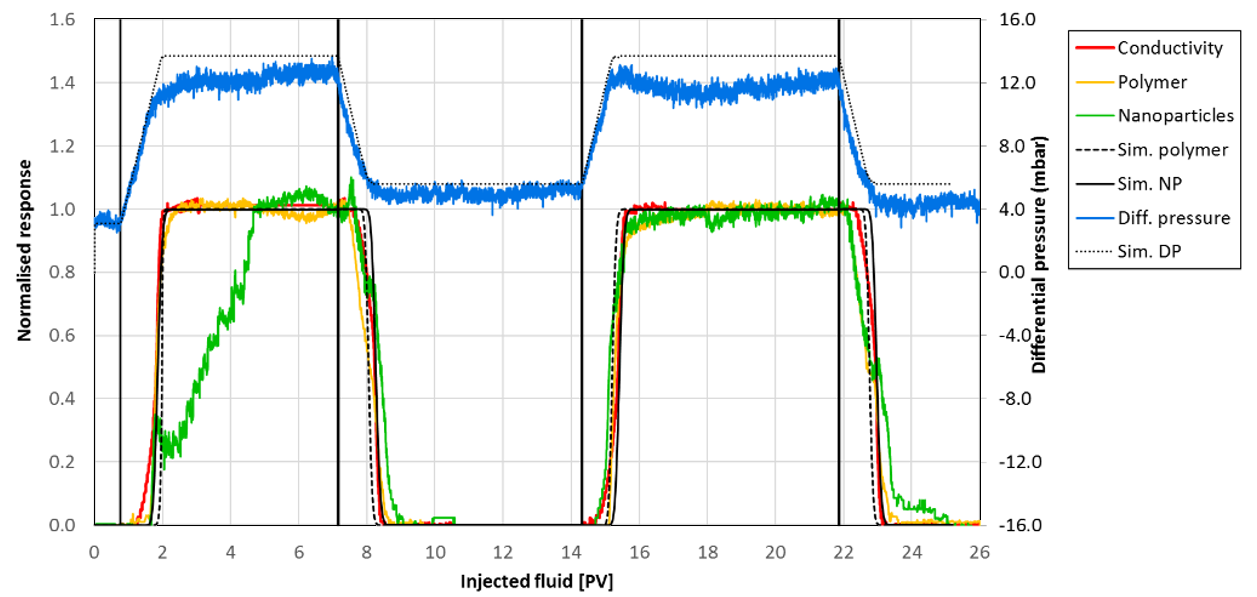
\includegraphics[width=\textwidth]{fig/simExpNP3.png}
    \caption{Comparison of experiment and simulation of co-injection of nanoparticles and polymer (Experiment 3 with Bentheimer). The nanoparticle response during the first injection slug in the experiment is assumed to be wrong. Conductivity measurements from the experiment and differential pressure over the core is also plotted.}
    \label{cht:simExpNP3}
\end{figure}

Experiments 4 – 6 follows the same schedule as experiment 1 – 3. Core material is now Berea sandstone with permeability around 0.3 Darcy and porosity around 19\% (see Table \ref{tab:ipvexp1}). From the experiments, it is apparent that the core is more heterogeneous than the Bentheimer sandstone and that early breakthrough and tailing occurs. The effect of heterogeneity cannot be modelled correctly in the 1D simulator and results from the simulations will have a more "piston like" displacement.

To compare the results from the developed 1D simulator with a commercial simulator and test the effect of heterogeneity, experiment 5 with injection of polymer into Berea sandstone has been simulated on 2D grids using ECLIPSE from Schlumberger. Three different models were constructed. One homogenous model with the same properties as used in the 1D model and two models with heterogenous permeability distribution. Permeability in the two heterogenous models varies between 100 and 400 mD, the first heterogenous model have constant permeability in layers (or tubes) while the second has a randomly distributed permeability (Figure \ref{cht:sim2dPerm}). 

\begin{figure}[h]
    \centering
    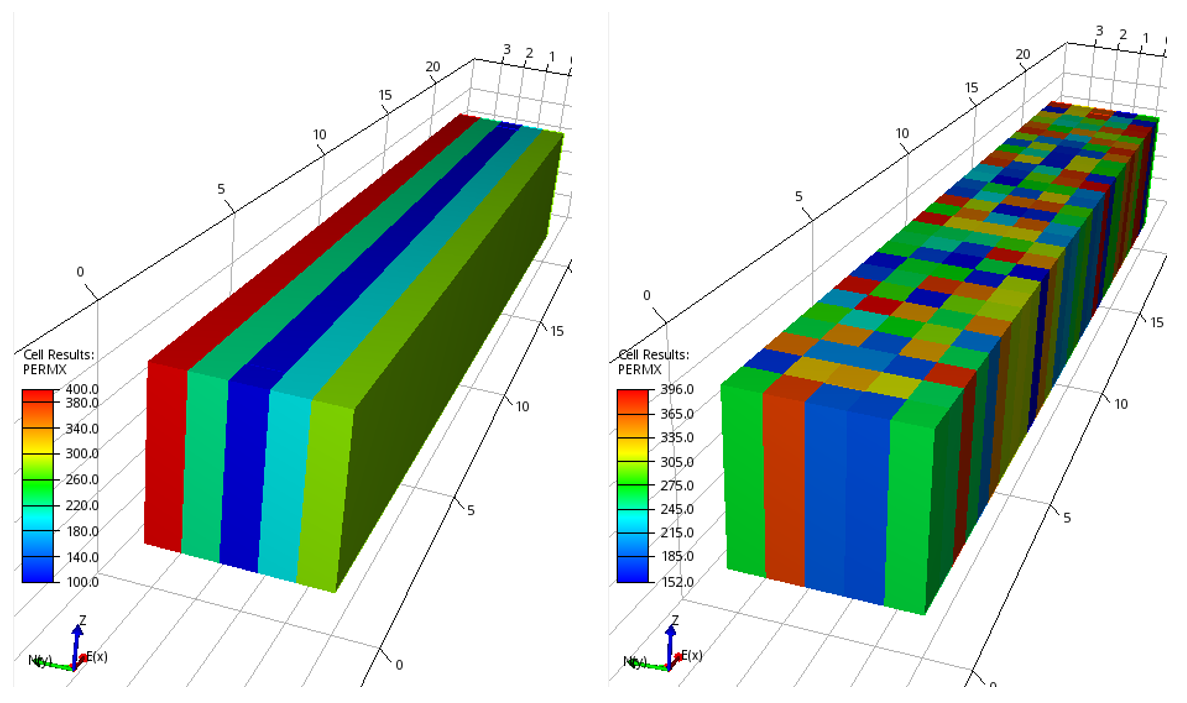
\includegraphics[width=\textwidth]{fig/sim2dPerm.png}
    \caption{Permeability distribution in the heterogenous 2D Eclipse models.}
    \label{cht:sim2dPerm}
\end{figure}

\enlargethispage{2cm} % add margin to bottom of this page
The ECLIPSE simulator has the functionality for modelling polymer injection in the aqueous phase and the same parameters as before for IPV, viscosity change as function of polymer concentration and adsorption of polymer, have been used. The results from the homogenous Eclipse simulation show a good match to the simulations from the developed 1D simulator (Figure \ref{cht:simEcl}).

\begin{figure}
    \centering
    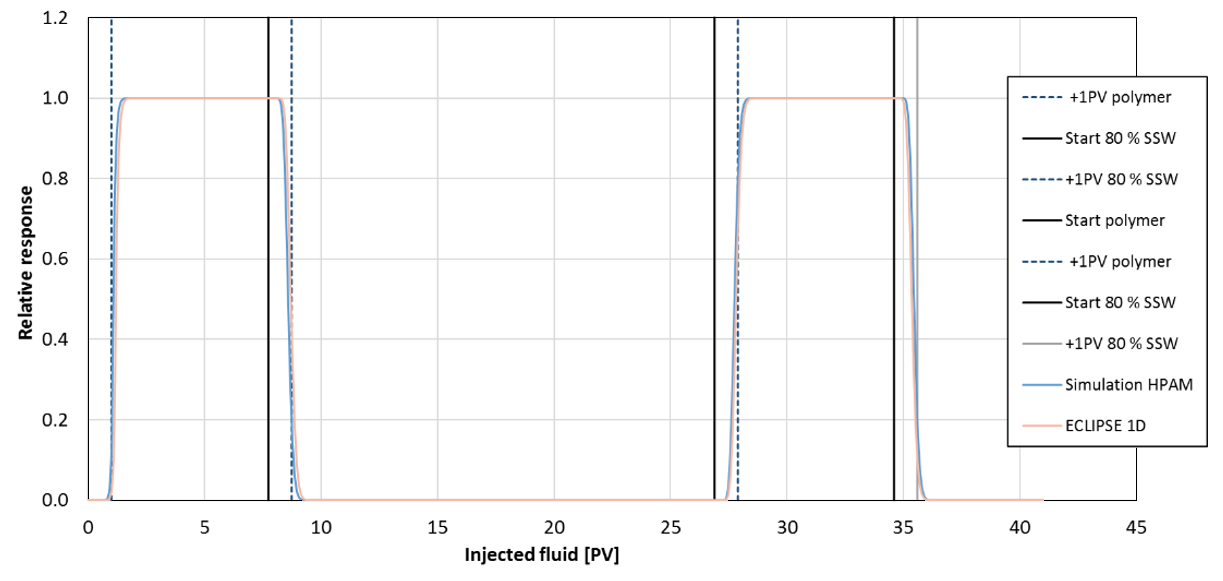
\includegraphics[width=\textwidth]{fig/simEcl.png}
    \caption{Comparison of polymer response between ECLIPSE and the developed simulator.}
    \label{cht:simEcl}
\end{figure}

\FloatBarrier

Results from adding simple heterogeneity to the ECLIPSE models are shown in Figure \ref{cht:simEclHet}. For the layered ``pipe" model a tail in the polymer response is apparent at SSW break through after the first and second polymer flood. This is an effect of polymer flowing in layers with different permeabilities. There is also a smoothing of the polymer front at break through. Similar effects can be seen in the random permeability model but not to the same degree.    

\begin{figure}
    \centering
    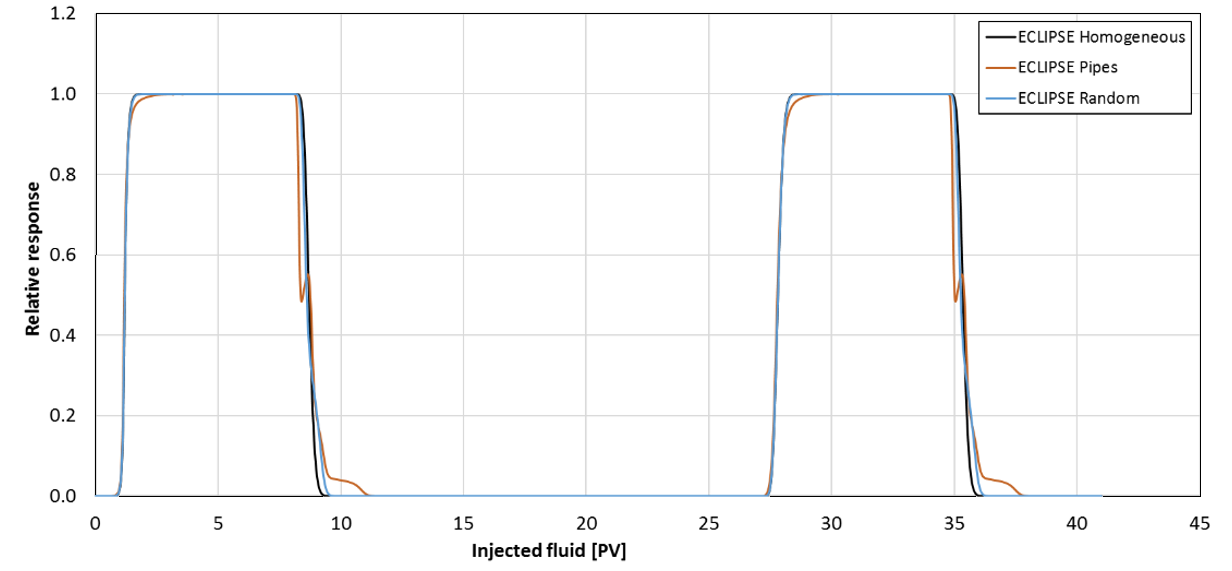
\includegraphics[width=\textwidth]{fig/simEclHet.png}
    \caption{Effect of heterogeneity in the ECLIPSE simulation models for polymer injection.}
    \label{cht:simEclHet}
\end{figure}

The effects of physical dispersion at the leading edge of the polymer slug and the fingering effects at the rear edge of the polymer slug is not implemented in the 1D simulator. Eclipse treats this with a Todd-Longstaff type mixing parameter,  $\omega$, for the effective water viscosity. The effective water viscosity is given as
\begin{equation}
    \mu_{p_\textit{eff}} = (\mu_m(C_p))^\omega \cdot \mu_p^{1-\omega}
\end{equation}
where the effective viscosity,  $\mu_{p_\textit{eff}}$, is a mix between the viscosity of a fully mixed polymer solution,  $\mu_m(C_p)$, and the viscosity of the solution at maximum polymer concentration,  $\mu_p$.  $\omega$ is the Todd-Longstaff mixing parameter which must be between 0 and 1.0. Figure \ref{cht:simEclMix} shows the polymer response in the homogeneous Eclipse model with mixing parameters 0.1, 0.5 and 1.0. Observe that using a mixing parameter less than one leads to dispersion in front and at the tail of the polymer slug.

\begin{figure}
    \centering
    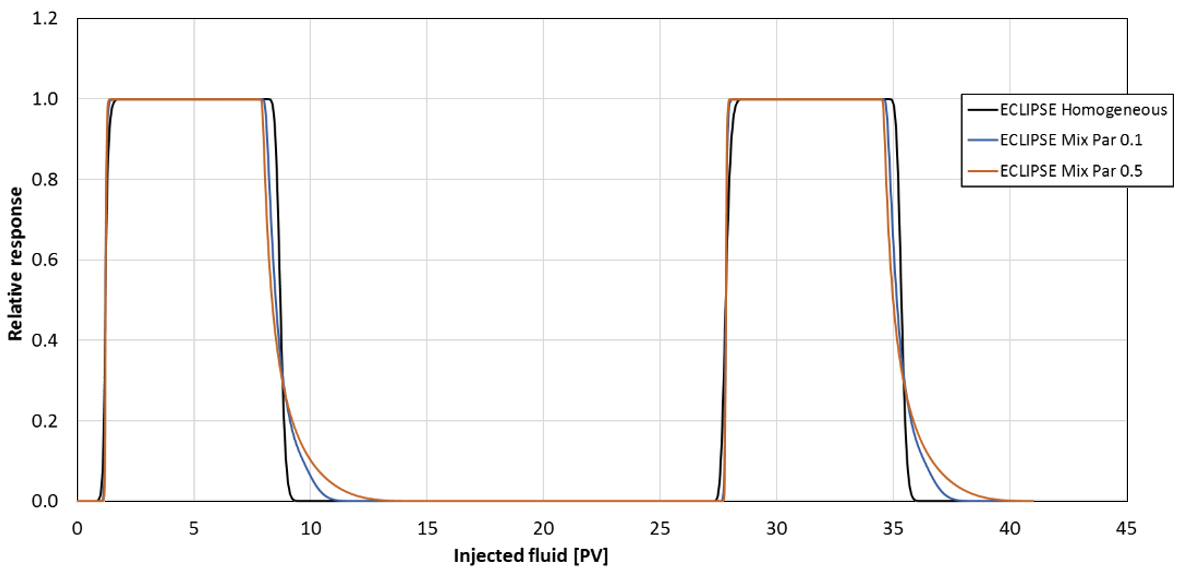
\includegraphics[width=\textwidth]{fig/simEclMix.png}
    \caption{Effect of using the mixing parameter for water viscosity in the ECLIPSE simulation models for polymer injection. }
    \label{cht:simEclMix}
\end{figure}

\section{Field scale modeling}
The full functionality of the simulator was tested by constructing a 100 m long simulation model with cross section 1 m$^2$. The simulation model has 1200 grid blocks, porosity and permeability was 0.24 and 2000 mD, respectively and the  IPV for polymer was set to 0.14. Otherwise, the parameters were as in experiment 3. Figure \ref{fig:largeScaleModel} shows an outline of the model.
\begin{figure}[h]
    \centering
    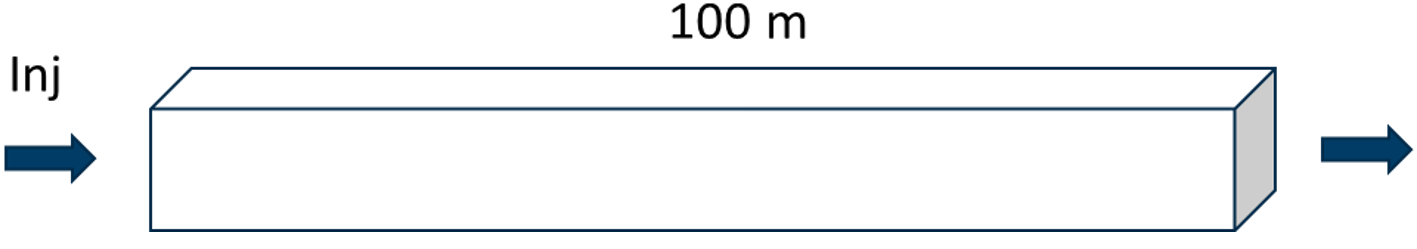
\includegraphics[width=\textwidth]{fig/largeScaleModel.png}
    \caption{Outline of the large-scale model. }
    \label{fig:largeScaleModel}
\end{figure}

Total pore volume (PV) of the model was 24 m$^3$ and an injection rate of 1 PV per 40 days were used (0.6 m$^3$/day). The schedule was set to inject a slug of 0.5 PV polymer and nanoparticle solution followed by 1.5 PV SSW. 

The applied age function for nanoparticles is shown in Figure \ref{cht:ageFunc} where nanoparticles start to crosslink the polymers at age 30 days. Full crosslinking effect for nanoparticles are reached after 33 days. Figure \ref{cht:hFunc} shows the two-variable function $h(C_p,C_n)$  reflecting the gel strength as function of polymer and nanoparticle concentrations.      

\begin{figure}[h] % figure 6.14
    \begin{subfigure}{.5\textwidth}
    \centering
    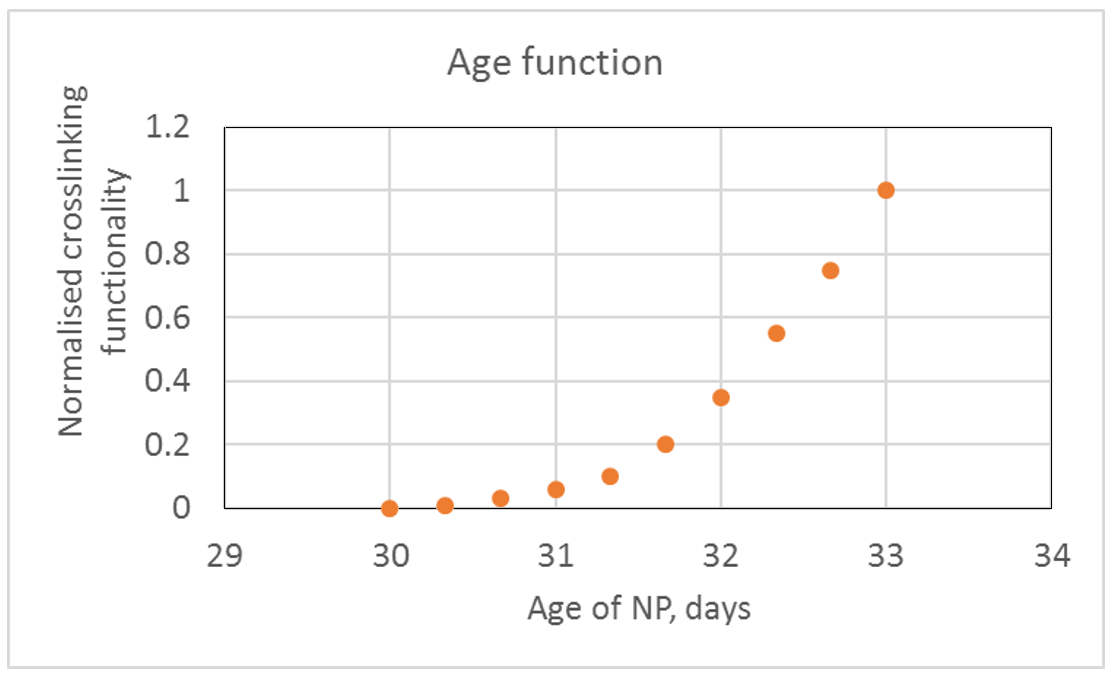
\includegraphics[width=\textwidth]{fig/ageFunc.png}
    \caption{}
    \label{cht:ageFunc}
    \end{subfigure}
    \\
    \begin{subfigure}{.5\textwidth}
    \centering
    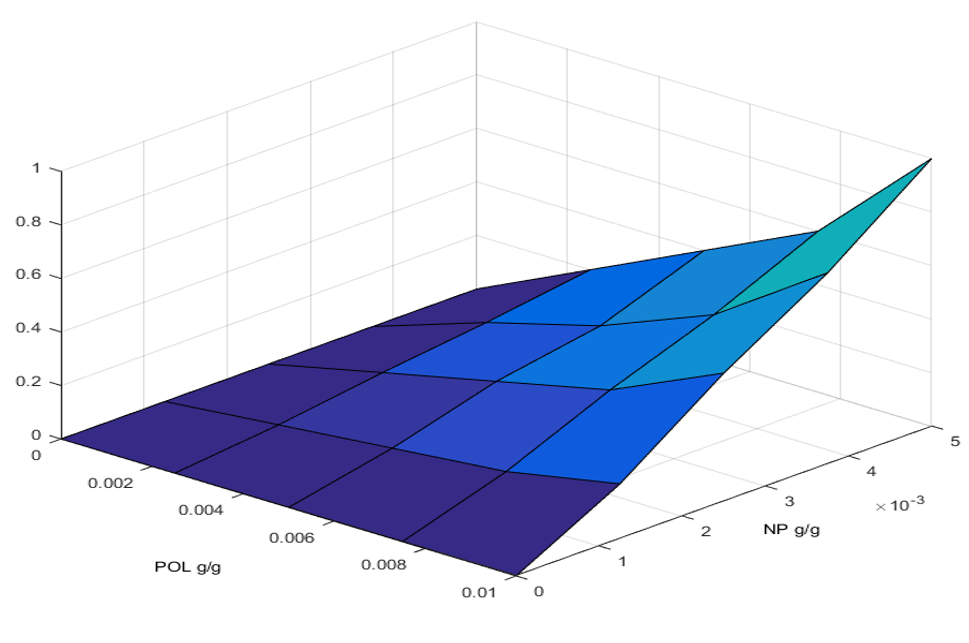
\includegraphics[width=\textwidth]{fig/hFunc.png}
    \caption{}
    \label{cht:hFunc}
    \end{subfigure}
    
    \caption{a) Age function for nanoparticles, $T_0$ is at 30 days and full crosslinking effect is reached at 33 days. b) $h$-function (see equation \ref{eq:ageEffect}), two parameter function of polymer and nanoparticle concentrations. }
    \label{cht:ageAndH}
\end{figure}

With the given nanoparticle age function the gelling should start at after 30 days, which corresponds to 75 m into the model. Maximum gel viscosity has been set to 50 cP to allow continued flooding of the 1D model after gel has formed. When gelling occurs in the model, a clear response on the differential pressure over the model should be noticed. Figure \ref{cht:pDiff} display differential pressure over the model and the relative concentrations of nanoparticle and polymer at the outlet of the model for injection of a) 0.5 PV polymer and nanoparticle solution and b) 0.25 PV polymer and nanoparticle solution followed by injection of SSW up to a total of 2 PV injected fluids. Both cases show an increase in differential pressure during solution injection due to increase in viscosity as function of polymer concentration. Reduction of effective permeability due to adsorption of polymer can be seen as a continued, but smaller increase in differential pressure until gelling occurs (at 0.75 PV injected or 75 m into the model) with a distinct increase in differential pressure. Observe that IPV and adsorption results in a splitting of the nanoparticle and polymer slugs and that for the case with slug size 0.25 PV only a smaller slug with high concentrations of both polymer and nanoparticles are produced at the outlet of the model. This is also reflected in a lower differential pressure over the model when gelling occurs.  

\begin{figure}[h] % figure 6.15
    \begin{subfigure}{.5\textwidth}
    \centering
    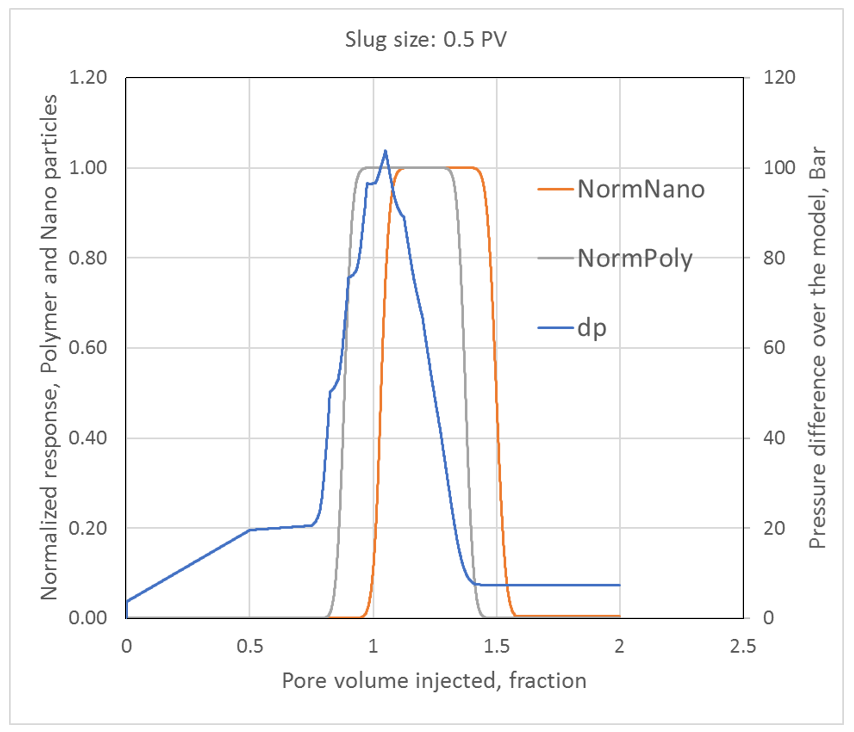
\includegraphics[width=\textwidth]{fig/pDiff1.png}
    \caption{}
    \label{cht:pDiff1}
    \end{subfigure}
    \\
    \begin{subfigure}{.5\textwidth}
    \centering
    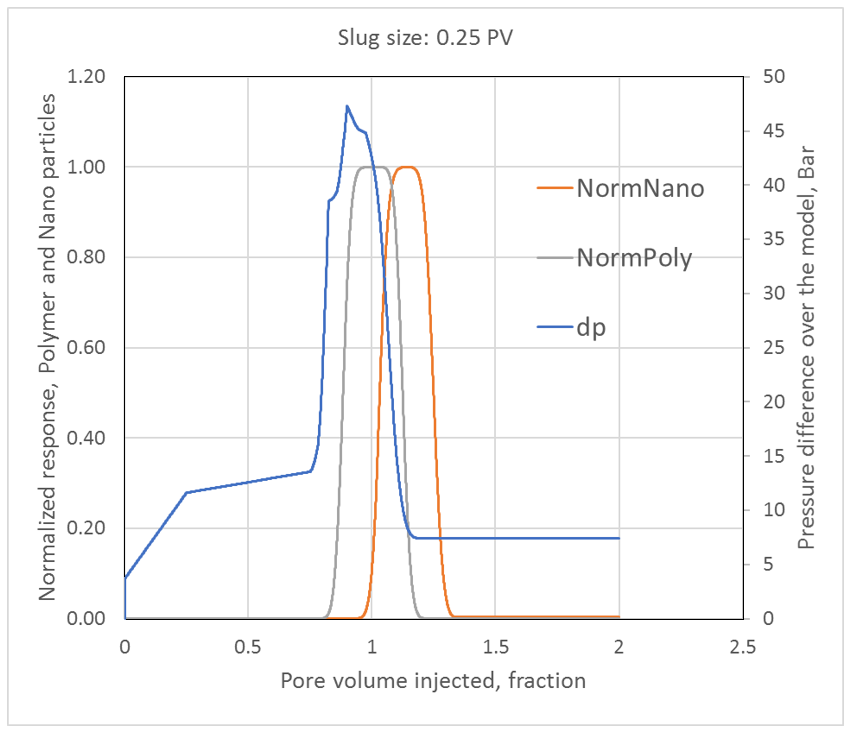
\includegraphics[width=\textwidth]{fig/pDiff2.png}
    \caption{}
    \label{cht:pDiff2}
    \end{subfigure}
    
    \caption{Differential pressure response for the large scale gelling simulation with a) injection of 0.5 PV polymer and nanoparticle slug and b) injection of 0.25 PV polymer and nanoparticle slug, both followed by SSW injection. }
    \label{cht:pDiff}
\end{figure}

\section{Conclusion}
Deep placement of gel in water flooded oil reservoirs may block channels with high water flow and divert the water into other parts of the reservoir. In order to get the gel constituents to the correct positions a delay in the gelling time up to weeks or months at elevated temperatures will be necessary. Further, the gel constituents must be environmentally acceptable. The objective of the HyGreGel project was to develop gel systems based on innovative chemistry taking nanoparticles into use and where the gelling time can be increased. Further, mechanisms for reaction and transport of the gel constituents should be described enabling modelling of deep gel placement in oil reservoirs.

A methodology for controlled gelation of partially hydrolysed polyacrylamide (HPAM) using hybrid nanoparticles with functional groups (FN particles) as cross-linkers has been developed. Several systems with different types of FN particles have been synthesized, characterized and tested. Two different delay mechanisms were found.  Both FN particles with fully blocked reactive sites that were slowly activated by hydrolysis and partially deactivated FN particles could significantly delay the gelation rate, giving gelling times ranging from several days to several months in synthetic sea water at 80~\celsius.

A gel system based on partially modified FN particles has been tested in core flooding experiments. The resistance to water flow increased with aging time, ultimately giving a very strong gel. The chemical system used has a severe injectivity problem that must be solved, however.    

Use of polyelectrolyte complexes as a method for delayed gelation based on published
technology developed at Texas A\&M University has been tested. Delayed gelation was obtained at 50~\celsius~ but not at 80 ℃. When the original polycation was replaced  
active FN particles also being a polycation, and dextranesulphate was replaced with polyvinylsulphonate, a reduced rate of gelation at 80~\celsius~ was also obtained.  

A mathematical model of 1D two-phase flow with polymers and nanoparticles have been developed, implemented and tested. The formulation includes tracking the age distribution of the nanoparticles. This means that at each position and time, the composition of the nanoparticles with respect to age and concentration are given. The age composition of the particles in solution in turn affects the nanoparticles ability to crosslink and form gel. Results from the core flooding experiments with deactivated FN particles and polymer were used in the testing. Simulations have also been done using a synthetic data set where polymer viscosity depends on polymer concentration and the concentration and age of the injected nanoparticles (the time passed since injection).



The use of a selected type of deactivated FN particles for improving oil recovery during water flooding was tested in both water wet and neutral wet Berea cores. No improvements in the oil recovery were obtained, however.

A significant step towards enable hybrid material technology as a next generation of chemical EOR has been taken through the HyGreGel project. However, within the frame of the present project it has not been possible to follow all the topics involved in the technology to the end. Further research and development will be needed to optimize and improve the technology to the level needed for field testing. 


\section{Appendix: Description of the Numerical Model}
\subsection{Defining equations}
We consider an immiscible two-phase (water and oil) 1D model with injection of nanoparticles and polymer in solution with water, where capillary and gravitational forces are ignored. We will assume that polymer and sufficiently old nanoparticles forms gel, increasing the water viscosity significantly. The boundary conditions are given by specifying an (time dependent) input rate. 

\subsection{Conservation laws}
Mass conservation for oil and water read
\begin{equation} \label{eq:massConservation} % eq 5.1
    \phi\frac{\partial S_i}{\partial t}+\frac{\partial u_i}{\partial x} = 0,\quad i = o, w
\end{equation}
where $\phi$ is the constant porosity (porosity for oil and water), $S_i=S_i(x,t), i = o,w$ are the phase saturations and $u_i, i=o,w$ are the phase volumetric fluxes. These fluxes are given by Darcy’s law
\begin{equation} \label{eq:fluxes} % eq 5.2
    u_i= -k\frac{k_{ri}}{\mu_i}\frac{\partial P}{\partial x},\quad i = o, w
\end{equation}
where $P=P(x,t)$  is the pressure and $k$ is the absolute permeability. Here absolute permeability is a tabulated function of absorbed polymer concentration. Furthermore, $k_{ri}, i = o, w$ are the relative permeabilities to oil and water, which are functions of water saturation. In the present formulation, these relative permeabilities are of Corey type
\begin{subequations}
\begin{eqnarray}
 k_{rw}(S_w)=k^0_{rw}(\frac{S_w-S_{wi}}{1-S_{wi}-S_{or}})^{\alpha_w} ,\\
    k_{ro}(S_w)=k^0_{ro}(\frac{1-S_{or}-S_{w}}{1-S_{wi}-S_{or}})^{\alpha_o} ,
\end{eqnarray}
\end{subequations}
where $S_w\in [S_{wi}, 1-S_{or}]$. Here $S_{wi}$ and $S_{or}$ and are the irreducible water saturation and the residual oil saturation, $k^0_{ri}, i=o,w$  are the endpoint relative permeabilities, and , $\alpha_w$ and $\alpha_o$  the Corey exponents for water and oil. The oil viscosity $\mu_o$ is assumed constant, while the water viscosity $\mu_w$ will be a function of nanoparticle and polymer concentration, the nanoparticle age profile, as well as the flow rate. The calculation of water viscosity is presented in the next section.
Mass conservation of nanoparticles and polymers are given by 
\begin{equation} \label{eq:massConsNPpol} % eq 5.3
    \frac{\partial}{\partial t}(C_i\phi^{(i)}S_w + C_{ai}(1-\phi^{(i)})\rho_r)+ \frac{\partial}{\partial x}(C_i u_w) = 0, \quad i = n, p
\end{equation}
where $C_i=C_i(x,t), i=n,p$ are nanoparticle and polymer concentrations (molar or by weight), $C_{ai}=C_{ai}(C_i), i=n,p$ , are the adsorbed concentrations per mass of the rock for nanoparticles and polymers, $\phi^{(i)}, i=n,p$ , the porosities (accessible pore spaces) for nanoparticles and polymers, and finally, $\rho_r$ is the rock mass density. As indicated, the adsorbed concentrations are functions of their respective concentrations in the water phase, where the components can desorb or not depending on input choice. Thus, in case of no desorption, the adsorbed concentration is a hysteretic quantity.   
In addition to calculating the saturations and concentrations, we need to keep track of the local age profiles of the nanoparticles, both the age profile in the water phase and the age profile of the adsorbed nanoparticles (the adsorbed age profiles are needed if nanoparticles can desorb). This age tracking is realized by formulating a conservation scheme for nanoparticles of the same age.   

Let  $p(x,t;\tau)$ denote the age distribution of nanoparticles in solution at position  and time  . That is, 
\begin{equation*}
    p(x,t;\tau)\Delta\tau
\end{equation*}
is the fraction of nanoparticles having age in the interval $[\tau, \tau+\Delta\tau]$  at position $x$ and at time $t$. Thus $p(x,t;\tau)\geq 0$ and $\int_{0}^{\infty}{p(x,t;\tau)d\tau}=1$ . In case all nanoparticles at a location have aged more than a maximal age $T_1$, the age where maximal gel strength can be achieved, the age profile is given by the delta function $\delta(\tau-T_1)$. The age distribution of adsorbed nanoparticles at position $x$ at time $t$ is similarly given by $q(x,t;\tau)$. Thus, the total concentration of nanoparticles per bulk volume of age  $[\tau, \tau+\Delta\tau]$ at position $x$ at time $t$ is
\begin{equation}
    \left(p(x,t;\tau)C_n(x,t)\phi^{(i)}S_w(x,t)+q(x,t;\tau)C_{an}\left(C_n(x,t)\right)(1-\phi^{(n)})\rho_r\right)\Delta\tau
\end{equation}
The flux of nanoparticles of this age is
\begin{equation}
    p(x,t;\tau)C_n(x,t)u_w(x,t)\Delta\tau
\end{equation}
Thus, we can set up the conservation law for nanoparticles of age $[\tau, \tau+\Delta\tau]$  for determining the   $t$-evolution of $p(x,t;\tau)$ and $q(x,t;\tau)$. Exactly how this is realized will be described in the section describing the numerical realization of the mathematical model.

\subsection{Water viscosity}
The water viscosity is expressed as
\begin{equation}
    \mu_w=(1-\nu)\mu^p_w + \nu\mu_w^{\max}
\end{equation}
where $\mu^p_w$ is the water viscosity with only polymer present, $\mu_w^{\max}$ is the (constant) maximal possible value for water viscosity corresponding to maximal gel strength. $\nu\in[0,1]$ is an interpolator depending on nanoparticle and polymer concentrations and the age profile $p$, where  $\nu=0$ corresponds to no gelling, and $\nu=1$  signifies maximal gel strength.

The water viscosity with only polymer present is given by
\begin{equation}
    \mu_w^p=\mu_w^0 a(C_p) s(C_p, q_w),
\end{equation}
where $\mu_w^0$ is the water viscosity with no polymer present, $a (C_p)$ is the viscosity increase factor due to presence of polymer with no shear-thinning, while $s(C_p, u_w)$ is the viscosity decrease factor due to shear thinning. Note that the shear-thinning factor $s(C_p, u_w)$ is calculated explicitly in the numerical formulation. The two functions $a (C_p)$ and $s(C_p, u_w)$ are tabulated input parameters and can either be measured directly or calculated from some type of assumed functional form. The approach for defining the water viscosity as a function of polymer concentration resembles the fully mixed case for the Todd-Longstaff formulation \citep{slb2015}.   

The interpolator (signifying degree of gelling) is given by
\begin{equation} \label{eq:ageEffect} % eq 5.8
    \nu=h(C_n,C_p) \int^{T_1}_{0}m(\tau)p(x,t;\tau)d\tau
\end{equation}
where $h(C_n,C_p)$ is a tabulated function, and $m(\tau)$ a weight function defining how the age of the nanoparticles influence gel strength. The (normalized) function $m(\tau), \tau\in[0,T_1]$, measures the increase in water viscosity (that is interpolator value) as a function of nanoparticle aging. Typically $m(\tau)=0$ for $\tau\in[0,T_0]$,  $m^\prime(\tau)>0$ for $\tau\in\langle T_0, T_1\rangle$ , and $m(T_1)=1$ as illustrated in Figure \ref{fig:weightFunc}.

\begin{figure}[h]
    \centering
    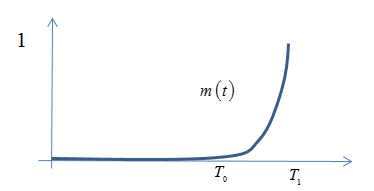
\includegraphics[width=.85\textwidth]{fig/weightFunc.png}
    \caption{Weight function signifying that gelling is initiated when nanoparticles have age $T_0$ and gelling reach maximal strength at age $T_1$}
    \label{fig:weightFunc}
\end{figure}

Consequently, the interpolator  $\nu$ is zero when all nanoparticles have aged less than  $T_0$. When all nanoparticles have aged more than  $T_1$, the age profile $p$ is set to  $\delta(\tau-T_1)$ , meaning that the integral in (\ref{eq:ageEffect}) satisfies $\int^{T_1}_{0}m(\tau)p(x,t;\tau)d\tau=1$ , giving the maximal value for this integral. We will refer to the integral in (\ref{eq:ageEffect})  as \textit{the age effect} (at position $x$ at time $t$ ). The function $m(\tau)$ must be measured or estimated keeping the nanoparticle and polymer concentrations constant. At this stage, we have assumed  $m(\tau)$ is independent of concentrations, but it would be straightforward to extend this function to depend on more variables. The other factor in (\ref{eq:ageEffect}), $h(C_n,C_p)$ , would reflect the gel strength as a function of the concentrations when all nanoparticles have the same age, and must be measured or estimated from more basic principles. At maximal concentrations, it is assumed that $h=1$ , while $h(C_n,C_p)=0$ when either of the concentrations are zero (i.e. no gel forms). Thus, when all nanoparticles have aged more than $T_1$, and when the nanoparticle and polymer concentrations sufficiently high (i.e. when $h(C_n,C_p)=1$ ), the interpolator is unity giving maximal value for water viscosity.

\subsection{Numerical realization, a summary}
It is important to formulate a numerical scheme that is as stable as possible. Consequently, the coupled conservation laws for water saturation, polymer-, and nanoparticle concentrations are solved numerically using (mainly) an implicit scheme. As the model is spatially 1D, not too many numerical grid blocks are needed, even for a fine spatial resolution. Few grid blocks also allow for using a small maximal time step without forbiddingly long simulations time. Therefore, the inherited numerical diffusion in implicit schemes can be limited by demanding short time steps, and using a first order implicit scheme (backward Euler) is sufficient for obtaining satisfactory precision. Also, the 1D formulation results in a block structured Jacobi matrix (tri-block diagonal) in the Newton iterations, allowing for a generalization of the well-known explicit solution of linear equations when the coefficient matrix is tri-diagonal. Consequently, the solver for linear equations is non-iterative, very robust, and fast. 

Not all terms are treated implicitly. The age effect $\int^{T_1}_{0}m(\tau)p(x,t;\tau)d\tau$ is updated at the end of the time step, meaning that only the factor $h(C_n,C_p)$ in (\ref{eq:ageEffect}) is treated implicitly. The age distributions $p$ and $q$ are also recalculated at the end of the time step using “mass conservation” for nanoparticles of the same age, and then adding the time step length to the age of all present nanoparticles. Incidentally, problems were encountered when solving for the “mass conservation” of the variously aged nanoparticles.  An explicit scheme for solving for the transport of various aged nanoparticles rendered unstable, while a fully implicit scheme gave rise to forbiddingly high numerical dispersion. However, by using an explicit upstream and implicit downstream seems to give excellent profiles for the age distributions. A Google search for this explicit upstream, implicit downstream approach actually revealed one single previous paper on this topic \citep{Flatten2008}. 

We first describe how the conservation equations are solved numerically, and then define how the age profiles are updated and how the age effect is calculated.

\subsection{Conversion equations}
The phase mobilities are defined as
\begin{equation}
    \lambda_i = \frac{k_{ri}}{\mu_i}, \quad i=w,o
\end{equation}
First, we eliminate the pressure from the system of equations to obtain the standard Buckley-Leverett formulation. Adding the two equations given by (\ref{eq:massConservation}), and using $S_w+S_o=1$ we obtain $\frac{\partial}{\partial x}(u_w+u_o)=0$  which means that $u_T=u_w+u_o=u_T(t)$  , where $u_T$ is the total volumetric flux defined by the boundary conditions. From (\ref{eq:fluxes}) we then solve for the pressure (-derivative)
\begin{equation} \label{eq:pressureDerivative} % eq 5.9
    \frac{\partial P}{\partial x} = -\frac{u_T}{k\lambda_T}
\end{equation}
where  $\lambda_T=\lambda_w+\lambda_o$ is the total mobility. In particular, (\ref{eq:pressureDerivative}) is used for calculating the pressure after a converged time step. Note that the absolute permeability only enters in the model through (\ref{eq:pressureDerivative}) (not in the system of equations we solve) when the pressures are calculated for reporting purposes. Indeed, when using rate controlled boundary conditions and incompressible flow, the pressure is not “an issue” as it is eliminated by (\ref{eq:pressureDerivative}) from the set of equations. Also, note that total volumetric flux $u_T(t)$ in (\ref{eq:pressureDerivative}) is given from the input data, not calculated. From (\ref{eq:massConservation}) with  $i=w$ we then obtain
\begin{equation} \label{eq:fractionalFlow} % eq 5.10 
    \phi\frac{\partial S_w}{\partial t}+u_T(t)\frac{\partial f_w}{\partial x} = 0
\end{equation}
where $f_w=\frac{\lambda_w}{\lambda_T}$ is the fractional flow of water. The mass conservation equations for nanoparticles and polymers given by (\ref{eq:massConsNPpol}) are then expressed as
\begin{equation} \label{eq:longMassConservation} % eq 5.11
    \frac{\partial}{\partial t}\left( C_k\phi^{(k)}S_w + C_{ak}(C_k)(1-\phi^{(k)}) \rho_r \right) + u_T(t) \frac{\partial}{\partial x}(C_k f_w)=0, \quad k=n,p
\end{equation}
The three equations given by (\ref{eq:fractionalFlow}) and (\ref{eq:longMassConservation}) are coupled and non-linear, and are solved for $S_w$, $C_n$ and $C_p$  using Euler’s backward method, with the explicit exceptions referred to earlier.

Given  $\Delta x$ and $\Delta t$ ($\Delta t$  varies in general for different time steps, while $\Delta x$ is assumed constant) at time $t=t^n$ , we let $S_w(i\Delta x, t_n+\Delta t) \approx S_i^{n+1}$ , and similarly for the other space and/or time dependent variables. Equation (\ref{eq:fractionalFlow}) becomes
\begin{multline}% eq 5.12
    E_i \left(S^{n+1}_{i-1}, C^{n+1}_{\textit{NP}, i-1}, C^{n+1}_{pol, i-1}, S^{n+1}_{i}, C^{n+1}_{\textit{NP}, i}, C^{n+1}_{pol, i}\right)  = \\ \phi\frac{S^{n+1}_{i}-S^{n}_{i}}{\Delta t} +u_T^{n+1}\frac{f_i^{n+1}\left(S^{n+1}_{i}, C^{n+1}_{\textit{NP}, i}, C^{n+1}_{pol, i}  \right) - f_{i-1}^{n+1}\left(S^{n+1}_{i-1}, C^{n+1}_{\textit{NP}, i-1}, C^{n+1}_{pol, i-1}  \right)}{\Delta x}  = 0 \\
    \quad
\end{multline} 
where we have dropped the $w$  index for water saturation and fractional flow. In simulations, the time step is such that the total rate  $u_T$ is constant in the corresponding time interval. We have assumed the direction of flow is with increasing spatial index value $i$ , and the water fractional flow is as indicated calculated using upstream weighted mobilities. As discussed, the water viscosity, and therefore the water fractional flow $f$, is not entirely implicitly calculated, as the age-profiles $p$ and the shear-thinning effect are treated explicitly.

The flux term in equation (\ref{eq:longMassConservation}) is also given by upstream weighting (assuming flow in direction of increasing index $i$ )
\begin{equation}
\begin{split}
    F_{k,i}\left(S^{n+1}_{i-1}, C^{n+1}_{\textit{NP}, i-1}, C^{n+1}_{pol, i-1}, S^{n+1}_{i}, C^{n+1}_{\textit{NP}, i}, C^{n+1}_{pol, i}\right) = u_T^{n+1} \frac{C^{n+1}_{k,i} f^{n+1}_{i} - C^{n+1}_{k,i-1} f^{n+1}_{i-1}}{\Delta x},\\  k=n,p \\ \quad
\end{split}
\end{equation}
The time derivative of the capacity term is approximated by
\begin{multline}
    G_{k,i}\left(S^{n+1}_{i}, C^{n+1}_{k,i}\right) = \\ 
    \phi^{(k)} \frac{C^{n+1}_{k,i} S^{n+1}_{i} - C^{n}_{k,i} S^{n}_{i}}{\Delta t} + \left(1-\phi^{(k)}\right) \rho_r 
    \frac{C_{ak} \left(C^{n+1}_{k,i}\right) - C_{ak} \left(C^{n}_{k,i}\right)}{\Delta t} U \left(C^{n+1}_{k,i} - C^{n}_{k,i}, w_k \right)
    ,\\ k=n,p \\ \quad
\end{multline}
where
\begin{equation*}
\begin{split}
    U(x,w) &= 1     \quad \text{if } w=0 \text{ \& } x\geq0 \text{, or if } w=1 \\
    U(x,w) &= 0     \quad \text{if } w=0 \text{ \& } x<0 
\end{split}
\end{equation*}
Here  $w_k=1$ if desorption can occur for component $k, (k=n,p)$, and $w_k=0$  if desorption does not occur.

As the model presently allows only water to be injected, we have  $q_T^{n+1}=\frac{Q_w^{n+1}}{A}$, where $Q_w^{n+1}$ is the given volumetric injection rate for water in the time interval $\left[t^n,t^{n+1}\right]$ , and where $A$ is the cross sectional area of the porous medium. Furthermore $f^{n+1}_0=1$,  $C^{n+1}_{k,0}=C^{n+1}_{k,inj}$, $k=n,p$, where $C^{n+1}_{k,inj}$ is the given injection concentration of component $k$ in the time interval $\left[t^n,t^{n+1}\right]$, and is constant during a time step. Let $n_x$  denote the number of grid blocks. For $i=1,2,...,n_x$, we then we have the $3n_x$  algebraic equations
\begin{equation}
    E_i \left(S^{n+1}_{i-1}, C^{n+1}_{\textit{NP}, i-1}, C^{n+1}_{pol, i-1}, S^{n+1}_{i}, C^{n+1}_{\textit{NP}, i}, C^{n+1}_{pol, i}\right)  = 0, % eq 5.15
\end{equation}
\begin{equation}
    G_{\textit{NP}, i} \left(S^{n+1}_{i}, C^{n+1}_{\textit{NP}, i}\right)+ F_{\textit{NP}, i} \left(S^{n+1}_{i-1}, C^{n+1}_{\textit{NP}, i-1}, C^{n+1}_{pol, i-1}, S^{n+1}_{i}, C^{n+1}_{\textit{NP}, i}, C^{n+1}_{pol, i}\right) =0, % eq 5.16
\end{equation}
\begin{equation}
    G_{\textit{pol}, i} \left(S^{n+1}_{i}, C^{n+1}_{\textit{pol}, i}\right)+ F_{\textit{pol}, i} \left(S^{n+1}_{i-1}, C^{n+1}_{\textit{NP}, i-1}, C^{n+1}_{pol, i-1}, S^{n+1}_{i}, C^{n+1}_{\textit{NP}, i}, C^{n+1}_{pol, i}\right) =0, % eq 5.17
\end{equation}
for the $3n_x$ unknowns $S^{n+1}_{i}, C^{n+1}_{\textit{NP}, i}, C^{n+1}_{pol, i}, i=1,2,...,n_x$.

Solving this set of non-linear equations requires use of Newton’s method for systems of equations, which again requires a new Jacobi matrix at each Newton iteration. The $3n_x \times 3n_x$   Jacobi matrix is sparse and block diagonal where the block matrices are generally $6\times6$  matrices. Due to this structure, Gauss-elimination does not destroy the sparse structure, and also the number of arithmetic operations in the Gauss-elimination only grow linearly with $n_x$. 

We will not write down the explicit formula for the Jacobi matrix as used in the computer code, but report that the Newton iteration shows excellent second order convergence using  $S^{n}_{i}, C^{n}_{\textit{NP}, i}, C^{n}_{pol, i}, i=1,2,...,n_x$   as initial guess in the iteration, which actually validates the expressions obtained and used for the various partial derivatives needed for forming the Jacobi matrix.

One can also analyze the explicit expression for the matrix to conclude that the Jacobi matrix is always not near singular, and no attempt have been made at this stage for calculating the condition number for the matrix.

It is important that  $C^{n+1}_{\textit{NP}, i}$ and $C^{n+1}_{pol, i}$ are scaled in the system of equations. This gives contributions from saturations and concentrations equal footing in the calculation of the residual in each Newton iteration.

\subsection{Updating age profiles}
At each position, and at each time step, the nanoparticles in solution and the adsorbed nanoparticles each have their own age profile $p$ and $q$. These age profiles are probability distributions on the interval $[0,T_1]$, i.e. $p\geq0$  and $\int^{T_1}_0 p(x,t;\tau)d\tau=1$  , and likewise for  $q$. No gelling (cross-linking) can occur before nanoparticles reach the minimum gelling age  $T_0$. Maximally strong gel may form at a given position and time when all the nanoparticles in solution have reached age $T_1$ (if also $h(C_n,C_p)=1$) the water reaches its maximal viscosity, see (\ref{eq:ageEffect})).

The numerical representations of $p(x,t;\tau)$ and $q(x,t;\tau)$ are given as follows: At time $t=t^n$ we let
\begin{equation}
    p(i\Delta x,t^n;\tau^r)=p^{n,r}_i, \quad i=1,2,...,n_x, \quad r=1,2,...,m^n,
\end{equation}
where $m^n$ is the number of ages at time $t^n$ , and similarly for $q$. The age profile resolution $\tau^1,\tau^2,...,\tau^{m^n}$ is dynamical, but the  $\tau$-resolution is the same for every position at a given time, both for $p$ and $q$.

At early times in the simulation, the list of ages, $\tau^1=t^n-t^{n-1},\tau^2=t^n-t^{n-2},...,\tau^{n-1}=t^n-t^1, \tau^{n}=t^n$, is defined by the length of the time steps. When the (user defined) maximum number of ages is obtained, the list of ages is recalculated. The maximal number of ages with $\tau^k<T_0$  is a given input value, and the same applies for the maximal numbers of ages for  $T_0\leq\tau^k\leq T_1$. When the maximum number of ages is reached, either ages younger than  $T_0$, or for ages in the interval $[T_0,T_1]$, the ages are redistributed evenly, and the age fractions $p$ and $q$ corresponding to the new list of ages recalculated to match the previous representation of $p$ and $q$. The recalculation of $p$ and $q$ uses linear interpolation for obtaining new values of  $p^{n,k}_i$ and $q^{n,k}_i$, and a renormalization to ensure $\sum^{m_n}_{k=1} p_i^{n,k}\Delta\tau^k=1$  and  $\sum^{m_n}_{k=1} q_i^{n,k}\Delta\tau^k=1$. When all ages of the nanoparticles in solution are older than $T_1$, the age effect entering in Equation (\ref{eq:ageEffect}), $\int^{T_1}_{0} m(\tau)p(x,t;\tau)d\tau$ is simply set to unity.

Now, assume we have obtained $S^{n+1}_{i}, C^{n+1}_{\textit{NP}, i}, C^{n+1}_{pol, i}, i=1,2,...,n_x$ at time $t=t^{n+1}$ from solving the conservation equations. In addition, we know the age distributions $p^{n,k}_i$ and $q^{n,k}_i$ at time $t=t^{n}$.

The flux of nanoparticles having age in the interval $\left[\tau^k, \tau^{k+1}\right]$ is
\begin{equation}
    p(x,t;\tau)C_n(x,t)u_w(x,t)\Delta\tau = p(x,t;\tau)C_n(x,t)u_T(t)f_w(x,t)\Delta\tau
\end{equation}
To compute the  $x$-derivative we will adopt an explicit upstream, implicit downstream method. That is, we will let
\begin{multline}
    \frac{\partial}{\partial x} \left(p(x,t;\tau)C_n(x,t)u_T(t)f_w(x,t)\Delta\tau\right) \approx \\ \frac{u_T^{n+1}}{\Delta x} \left(p_i^{n+1,k}C_{n,i}^{n+1}f_i^{n+1}- p_{i-1}^{n,k}C_{n,i-1}^{n}f_{i-1}^{n}\right)\Delta\tau
\end{multline}
Thus,
\begin{equation} \label{eq:massNP} % eq. 5.19
    u_T^{n+1} \left(p_i^{n+1,k}C_{n,i}^{n+1}f_i^{n+1}- p_{i-1}^{n,k}C_{n,i-1}^{n}f_{i-1}^{n}\right)\Delta\tau A\Delta t
\end{equation}
approximates the mass (or molar) of nanoparticles in solution of with ages in the interval $\left[\tau^k, \tau^k+\Delta\tau\right]$  flowing out of grid block $\left[x_{i-1},x_i\right],i=1,2,...,n_x$ during the time step  $\left[t^n, t^n+\Delta t\right]$. Here $A$ is the cross-sectional area of the model. As previously discussed, any other way of realizing the  $x$-derivative in (\ref{eq:massNP}) leads to non-physical results, either highly unstable (using explicit both up- and downstream) or forbiddingly dispersive (using a full implicit formulation). 

Assume first that the mass of nanoparticles flowing out of the grid block is negative. Then the nanoparticle concentration increases locally, and consequently no adsorbed nanoparticles will desorb at this position. Therefore, the age profile of the adsorbed nanoparticles $q_i^{n,k}$ at time $t^n$ will not affect the new age profile  $p_i^{n+1,k},k=1,2,...,m_{n+1}$ of the nanoparticles in solution at time  $t^{n+1}$. The mass of nanoparticles with ages in the interval $\left[\tau^k, \tau^k+\Delta\tau\right]$ is
\begin{equation*}
    \left(p(x,t;\tau)C_n(x,t)\phi^{(n)}S_w(x,t) + q(x,t;\tau)C_{an}(C_n(x,t))(1-\phi^{(n)})\rho_r\right) \Delta\tau A\Delta x
\end{equation*}
Thus, numerically the change of mass for these particles during the time step $\left[t^n, t^n+\Delta t\right]$ is
\begin{multline} \label{eq:massChangeNP} % eq 5.20
    \bigg[\phi^{(n)}\left(p_i^{n+1,k}C_{n,i}^{n+1}S_i^{n+1}- p_{i}^{n,k}C_{n,i}^{n}S_{i}^{n}\right) +\\ \rho_r(1-\phi^{(n)}) \left(q_i^{n+1,k}C_{an}(C_{n,i}^{n+1})- q_{i}^{n,k}C_{an}(C_{n,i}^{n})\right)\bigg]
    \Delta\tau A\Delta x
\end{multline}
We can eliminate $q_{i}^{n+1,k}$ by noting that the increased mass of adsorbed nanoparticles at this time step is
\begin{equation*}
    \left(C_{an}(C_{n,i}^{n+1})- C_{an}(C_{n,i}^{n})\right)
    \rho_r\left(1-\phi^{(n)}\right) A\Delta x
\end{equation*}
Thus, the increased mass of absorbed nanoparticles (which all come from the nanoparticles in solution) with ages in the interval $\left[\tau^k, \tau^k+\Delta\tau\right]$ is
\begin{equation*}
    p_i^{n+1,k}\left(C_{an}(C_{n,i}^{n+1})- C_{an}(C_{n,i}^{n})\right)
    \rho_r\left(1-\phi^{(n)}\right) A\Delta x.
\end{equation*}
Writing down mass conservation for absorbed nanoparticles of this age we find
\begin{multline} \label{eq:elimiateQ} % eq 5.21
    p_i^{n+1,k}\left(C_{an}(C_{n,i}^{n+1})- C_{an}(C_{n,i}^{n})\right)
    \rho_r\left(1-\phi^{(n)}\right) A\Delta x + \\
    C_{an}(C_{n,i}^{n})\rho_r\left(1-\phi^{(n)}\right)q_i^{n,k} = \\
    C_{an}(C_{n,i}^{n+1})\rho_r\left(1-\phi^{(n)}\right)q_i^{n+1,k}A\Delta x 
\end{multline}
Using (\ref{eq:elimiateQ}) we can then eliminate $q_i^{n+1,k}$ in (\ref{eq:massChangeNP}). 

Thus, formulating the mass conservation for nanoparticles of age $\left[\tau^k, \tau^k+\Delta\tau\right]$ using (\ref{eq:massNP}) and (\ref{eq:massChangeNP}) (having eliminated  $q_i^{n+1,k}$) we simply obtain an explicit formula $p_i^{n+1,k}$. Then from (\ref{eq:elimiateQ}) we find the values for $q_i^{n+1,k}$.

Assume now that the mass of nanoparticles decreases at a given position during a time step, i.e. that (\ref{eq:massNP}) is positive. Then if the option for no desorption of nanoparticles is set, the age profile for the adsorbed nanoparticles stays the same (except that all the adsorbed nanoparticles age the amount of the time step), and $C_{an}(C_{n,i}^{n+1})- C_{an}(C_{n,i}^{n})=0$. Thus (\ref{eq:elimiateQ}) is satisfied, and $q_i^{n+1,k}=q_i^{n,k}$, and the mass conservation for $p_i^{n+1,k}$ can be solved directly.

If desorption of nanoparticles can occur, then (\ref{eq:elimiateQ}) still applies, and $p_i^{n+1,k}$ and  $q_i^{n+1,k}$ can be found as previously described for the case when (\ref{eq:massNP}) is negative. 

We also observe that the procedure for updating the age profiles is done independently for each $k$.

In (\ref{eq:massNP}) for $i=1$, the age profile for the injected nanoparticles, $p_0^{n,k}$, has $p_0^{n,1}=1$ and $p_0^{n,k}=0$ for $k\geq2$. That is, all injected nanoparticles have minimum age. Note that it is simple to modify the model to allow for a general user defined age profile of the injected nanoparticles.

When $p_i^{n+1,k}$ and $q_i^{n+1,k}$ have been determined, the ages the distributions represent are of course increased by one time step, and the  $k$-index shifted one up. In fact, when the user defined maximal number of ages is reached, the computer code will always recalculate the representations of the age profiles as previously described, since adding a new age will exceed the maximal number of ages.

Finally, the age profile $p_i^{n+1,k},k=1,2,...,m_{n+1}$,  is used for estimating the integral
\begin{equation}
    \int_{T_0}^{T_1} m(\tau)p(x,t;\tau)d\tau
\end{equation}
\textit{the age effect}.

Since $m$ and $p$ generally are represented with values at different nodes, we linearly interpolate $p$ to match the nodes where $m$ is given, and calculate the integral using the trapezoidal method. This value for the age effect is then used in the upcoming new time step, where the other parameters defining water viscosity are treated implicitly in this new next time step (except the shear thinning effect).

\subsection{Table based input}
A number of the functions needed for the model are table based allowing for input generality. These functions constitute part of the input for the model, and must be measured in the laboratory or estimated from physical principles. All tabulated functions are either functions of one or two variables. Numerical noise may result in function calls outside the given domain, which could lead to ambiguities and possible failure of simulation. For functions of a single variable (defined on an interval) the code will both interpolate and extrapolate linearly. However, the program issues a warning when it has to extrapolate a function outside its given domain, reporting which function and which out of domain argument value it extrapolates to.

Two-variable functions are defined on a rectangle $\big[a,b\big]\times\big[c,d\big]$. Two-variable functions are evaluated by successive linear interpolation. Concerning extrapolation outside the domain of definition, for an argument $(x,y)$ which both has $x\notin\big[a,b\big]$ and $y\notin\big[a,b\big]$, the error will be fatal, and the program stops. In case of membership in only one of the intervals, the code will extrapolate linearly and report a warning.

Also, the various derivatives of table defined functions are needed for the Jacobi matrix. The derivatives are piecewise constant, and are calculated consistently with the linear interpolation of function values. Regarding extrapolation of derivatives, the values of derivatives are simply extended constantly outside their domains, both the ordinary and the partial derivatives.

As mentioned so far, the Newton iterations behave excellent showing second order convergence. This indicates that the implemented formulation and evaluation of function values and derivatives of table based functions is sound and robust.   

 





% back matter
\newpage
\bibliography{ref}
\end{document}


